\documentclass[../main.tex]{subfiles}
\begin{document}
\setchapterimage[6.5cm]{Images/Flavours.png}
\setchapterpreamble[u]{\margintoc}
\chapter[Lectures by Prof. Nardecchia]{Lectures by Prof. Nardecchia\footnotemark[0]}
\labch{mn}
\section{CP Violation in the Standard Model}
For parity, charge conjugation and CP application, we have to keep in mind the following table:
\begin{table}[h]
    \centering
    {\renewcommand{\arraystretch}{1}
    \begin{tabular}{c|c|c|c}
    \hline
    \rowcolor{blue!30}Fields & $\hat{P}(x\xrightarrow[]{}\pazocal{P}x)$ & $\hat{C}$ & $\hat{CP}(x\xrightarrow[]{}\pazocal{P}x)$\\
    \hline
    $\overline{\Psi}\chi$ & $\overline{\Psi}\chi$ & $\overline{\chi}\Psi$ & $\overline{\chi}\Psi$\\
    $\overline{\Psi}_R\chi_L$ & $\overline{\Psi}_L\chi_R$ & $\overline{\chi}_R\Psi_L$ & $\overline{\chi}_L\Psi_R$\\
    $\overline{\Psi}_L\chi_R$ & $\overline{\Psi}_R\chi_L$ & $\overline{\chi}_L\Psi_R$ & $\overline{\chi}_R\Psi_L$\\
    $\overline{\Psi}\gamma^\mu\chi$ & $\overline{\Psi}\gamma_\mu\chi$ & $-\overline{\chi}\gamma^\mu\Psi$ & $-\overline{\chi}\gamma_\mu\Psi$ \\
    $\overline{\Psi}_L\gamma^\mu\chi_L$ & $\overline{\Psi}_R\gamma_\mu\chi_R$ & $-\overline{\chi}_R\gamma^\mu\Psi_R$ & $-\overline{\chi}_L\gamma_\mu\Psi_L$\\
    $\overline{\Psi}_R\gamma^\mu\chi_R$ & $\overline{\Psi}_L\gamma_\mu\chi_L$ & $-\overline{\chi}_L\gamma^\mu\Psi_L$ & $-\overline{\chi}_R\gamma_\mu\Psi_R$\\
    \hline
    \end{tabular}
    }
    \caption*{}
    \labtab{CP}
\end{table}\\
For every term there is a phase factor $e^{i(\phi_\chi-\phi_\Psi)}$ associated, for example we have the term $\overline{\Psi}\chi(x)\xrightarrow[]{\hat{CP}}e^{i(\phi_\chi-\phi_\Psi)}\overline{\chi}\Psi(\pazocal{P}x)$. Now we apply $\hat{CP}$ to all the relevant stuff we already know.
\[
\left\{
\begin{aligned}
&W_\mu^+(x)\to-e^{+i\xi_W}\pazocal{P}_\mu^\nu W_\mu^-(\pazocal{P}x)
&&G_\mu^a(x)\to-\eta_a\pazocal{P}_\mu^\nu G_\nu^a(\pazocal{P}x)\\   
&W_\mu^-(x)\to-e^{-i\xi_W}\pazocal{P}_\mu^\nu W_\mu^+(\pazocal{P}x) &&h(x)\to\eta_h h(\pazocal{P}x)\\
&Z_\mu(x)\to-\eta_Z\pazocal{P}_\mu^\nu Z_\nu(\pazocal{P}x) &&u_i\to e^{i\phi_{u_i}}\gamma^0C\overline{u}_i^T\\
&A_\mu(x)\to-\pazocal{P}_\mu^\nu A_\nu(\pazocal{P}x) &&d_i\to e^{i\phi_{d_i}}\gamma^0C\overline{d}_i^T
\end{aligned}
\right.
\]
At this point we ask ourselves whether the SM is \textbf{invariant} under $\hat{CP}$ or not. In other words, we would like to know if it is possible to find the parameters $\xi_W, \eta_Z, \eta_h, \phi_{u_i},$ and $\phi_{d_i}$ such that $\hat{CP}\pazocal{L}(x)\hat{CP}^\dagger=\pazocal{L}(\pazocal{P}x)$.\\
The Standard Model Lagrangian can be decomposed into: 
\[
\pazocal{L}_{\text{SM}}=\pazocal{L}_{\text{kin}}+\pazocal{L}_{\text{Higgs}}+\pazocal{L}_{\text{Yuk}}
\]
The typical term containing the $Z$ boson is in the form:
\[
\sum_{f=u,d;A=L,R}\overline{f}_A\gamma^\mu f_AZ_\mu g_A^f
\]
where $g_A^f$ are real and constant coefficients. We now apply $\hat{CP}$ to it: the fermions appear as bilinears and the phase is cancelled because there is $\overline{f}_Af_A$, so we just focus on the sign. Under $\hat{CP}$ we get:
\[
\overline{f}_A\gamma^\mu f_A\xrightarrow[]{}(-\overline{f}_A\gamma^\mu f_A)e^{i\phi_{f_A}}e^{-i\phi_{f_A}}
\]
For the $Z$ we have $-\eta_ZZ^\mu$, therefore in order to have the $Z$ boson term invariant under $\hat{CP}$ it has to be $\eta_Z=+1$.\\
We move to the Higgs: 
\[
\pazocal{L}_{\text{Higgs}}=-m_h^2h^2+\lambda vh^3+\lambda h^4
\]
The term $\sim h^3$ tells us that it has to be $\eta_h=+1$.\\
The Yukawa sector does not give us a relevant contribution:
\[
\hat{CP}\pazocal{L}_{\text{Yuk}}\hat{CP}^\dagger=\hat{CP}Y_fh\overline{f}f\hat{CP}^\dagger=\hat{CP}Y_fh\hat{CP}^\dagger\hat{CP}\overline{f}f\hat{CP}^\dagger
\]
We apply $\hat{CP}$ to the $h$ and get $\eta_h=+1$ as seen before, while $\overline{f}f$ gives a +1 sign so everything is fine.\\
We are now left with $\xi_W, \phi_{u_i}$ and $\phi_{d_i}$, i.e. the phases related to $W_\mu$, $u_i$ and $d_i$.
\[
\hat{CP}\left[\frac{g}{\sqrt{2}}W_\mu^+\overline{u}_L^i\gamma^\mu d^j_LV_{ij}+\frac{g}{\sqrt{2}}W_\mu^-\overline{d}_L^j\gamma^\mu u_L^iV_{ji}^*\right]\hat{CP}^\dagger
\]
We insert $\hat{CP}^\dagger\hat{CP}=\mathbb{1}$ in the expression above and what we find is:
\[
\frac{g}{\sqrt{2}}V_{ij}\left[-e^{+i\xi_W}(W^-)^\mu e^{i(\phi_{d_j}-\phi_{u_i})}\left(-\overline{d}_L^j\gamma_\mu u_L^i\right)\right]+\frac{g}{\sqrt{2}}V_{ji}^*\left[-e^{-i\xi_W}(W^+)^\mu e^{i(\phi_{u_i}-\phi_{d_j})}\left(-\overline{u}_L^i\gamma_\mu d_L^j\right)\right]
\]
In order to get CP invariance, it has to be 
\[
V_{ji}^*=V_{ij}\exp{i(\xi_W+\phi_{d_j}-\phi_{u_i})}
\]
Is it possible to fix these phases such that this combination becomes real?\\
The matrix $V\in\text{U}(3)$ has 9 parameters: 3 angles+6 phases. However, in our case we have only 7 parameters: 
\[
\overset{(1)}{\xi_W} \quad \overset{(3)}{\phi_{u_i}} \quad \overset{(3)}{\phi_{d_j}}
\]
Some of them turns out to be useless. In principle, we have infinite solutions corresponding to 2 unbroken symmetries: U$(1)_{\text{B}}$, in which $\phi_u=\phi_d$ so we cannot use that because there are 5 phases, and U$(1)_{\text{Q}}$, corresponding to electromagnetism with the phases in the ratio +1, $-2/3$, $-1/3$.\\
We want to find CP violation in the unbroken phase, so with massless fields. For $\pazocal{L}_{\text{kin}}+\pazocal{L}_{\text{Higgs}}$ we have a U$(3)^3$ symmetry: 
\[
\text{U}(3)_{Q_L}\times\text{U}(3)_{u_R}\times\text{U}(3)_{d_R}
\]
This symmetry is broken by adding $\pazocal{L}_{\text{Yuk}}$, but before adding this piece we define a new CP transformation, which includes the U$(3)^3$ operators, and ask whether $\pazocal{L}_{\text{Yuk}}$ is invariant under the generalized CP transformation defined as follow:
\[
\left\{
\begin{aligned}
&\hat{CP}Q_L^i\hat{CP}^\dagger=(K_L)^i_je^{i\phi_{Q_L^i}}\gamma^0C(\overline{Q}_L^j)^T\\
&\hat{CP}u_R^i\hat{CP}^\dagger=(K_u)^i_je^{i\phi_{u_R^i}}\gamma^0C(\overline{u}_R^j)^T\\
&\hat{CP}d_R^i\hat{CP}^\dagger=(K_d)^i_je^{i\phi_{d_R^i}}\gamma^0C(\overline{d}_R^j)^T
\end{aligned}
\right.
\quad 
K_L,K_u,K_d\in\text{U}(3)
\]
Consider now the Yukawa term relative to the up and down quarks:
\[
-H^c\overline{Q}_L^i(Y_u)_{ij}u_R^j-H\overline{Q}_L^i(Y_d)_{ij}d_R^j+\text{h.c.}
\]
Applying CP to that term gives us:\marginnote{The phases defined in the previous transformation get reabsorbed in the $K$ matrices.}
\[
-H^cQ_L^iK_L^\dagger(Y_u)_{ij}K_u\overline{u}_R^j-HQ_L^iK_L^\dagger(Y_d)_{ij}K_d\overline{d}_R^j+\text{h.c.}
\]
This can be seen as:
\begin{equation}
\labeq{p1}
\left\{
\begin{aligned}
&Y_u\xrightarrow[]{}K_L^\dagger Y_uK_u\stackrel{?}{=}Y_u^*\\
&Y_d\xrightarrow[]{}K_L^\dagger Y_dK_d\stackrel{?}{=}Y_d^*
\end{aligned}
\right.
\end{equation}
So far, we rephrased the question about CP invariance in: are there $K_L,K_u$ and $K_d$ such that the condition above holds true? This is the same as:
\begin{equation}
\labeq{p2}
\left\{
\begin{aligned}
&K_L^\dagger Y_uY_u^\dagger K_L=(Y_uY_u^\dagger)^*\\
&K_L^\dagger Y_dY_d^\dagger K_L=(Y_dY_d^\dagger)^*
\end{aligned}
\right.
\end{equation}
In fact, by using \refeq{p1} we can show that we get \refeq{p2}:
\[
K_L^\dagger Y_uY_u^\dagger K_L=\underbrace{K_L^\dagger Y_u{\color{red}K_u}}_{Y_u^*}\underbrace{{\color{red}K_u^\dagger}Y_u^\dagger K_L}_{(Y_u^*)^\dagger}=Y_u^*(Y_u^*)^\dagger=(Y_uY_u^\dagger)^* \quad \checkmark
\]
We just need to prove that $K_u=Y_u^{-1}K_LY_u^*$ is unitary:
\[
K_uK_u^\dagger=Y_u^{-1}K_L\underbrace{Y_u^*Y_u^T}_{=(Y_uY_u^\dagger)^*}K_L^\dagger(Y_u^{-1})^T=Y_u^{-1}K_LK_L^\dagger Y_uY_u^\dagger K_LK_L^\dagger(Y_u^{-1})^T=\mathbb{1} \quad \checkmark
\]
If CP is conserved, then \refeq{p2} holds true. Moreover, if CP is conserved we have that $\Tr{[H_u,H_d]^r}=0$ when $r$ is odd, where we have defined $H_u:=Y_uY_u^\dagger$ and $H_d:=Y_dY_d^\dagger$, which are hermitian. To prove the second statement, we compute:
\begin{align*}
K_L^\dagger[H_u,H_d]K_L&=K_L^\dagger H_uH_dK_L-K_L^\dagger H_dH_uK_L\\
&=(K_L^\dagger H_uK_L)(K_L^\dagger H_dK_L)-(K_L^\dagger H_dK_L)(K_L^\dagger H_uK_L)\\
&\underset{\mathclap{\tikz \node {$\uparrow$} node [below=1ex] {\footnotesize \refeq{p2} };}}{=}H_u^*H_d^*-H_d^*H_u^*=[H_u^T,H_d^T]=-[H_u,H_d]^T
\end{align*}
It follows that $\Tr{[H_u,H_d]}=-\Tr{[H_u,H_d]}=0$. This was the case for $r=1$, now we generalize to any value of $r$:
\begin{align*}
\left(K_L^\dagger[H_u,H_d]K_L\right)^r&=K_L^\dagger[H_u,H_d]K_LK_L^\dagger[H_u,H_d]K_L\dots K_L^\dagger[H_u,H_d]K_L\\
&=K_L^\dagger[H_u,H_d]^rK_L=(-1)^r\left([H_u,H_d]^T\right)^r
\end{align*}
It then follows that: 
\[
\Tr{K_L^\dagger[H_u,H_d]^rK_L}=\Tr{[H_u,H_d]^r}=(-1)^r\Tr{[H_u,H_d]^r}
\]
This tells us that if we have a $r$ odd such that $\Tr{[H_u,H_d]^r}\neq0$, CP is violated. For $N_F=3$, we have that CP violation$\Rightarrow\Tr{[H_u,H_d]^3}=0$, while in all the other cases we just have $\Tr{[H_u,H_d]^3}\neq0\Rightarrow$CP violation. We can explicitly compute it for $r=3, N_F=3$:
\[
\Tr{[H_u,H_d]^3}=6i(y_t^2-y_c^2)(y_t^2-y_u^2)(y_c^2-y_u^2)(y_b^2-y_s^2)(y_b^2-y_d^2)(y_s^2-y_d^2)J
\]
$J$ is the Jarlskog invariant and it is used to quantify the amount of CP violation\marginnote{When pronouncing \textit{Jarlskog}, you might accidentally summon a demon in the extra-dimension (bad thing).}. The global U$(3)^3$ symmetry given by:
\[
\text{G=U$(3)_{Q_L}\times$U$(3)_{u_R}\times$U$(3)_{d_R}$}
\]
which comes from $\pazocal{L}_{\text{kin}}+\pazocal{L}_{\text{Higgs}}$, gets broken into H=U$(1)_{\text{B}}$ when we add $\pazocal{L}_{\text{Yuk}}$. We have seen that the Yukawa sector takes the form:
\[
\pazocal{L}_{\text{Yuk}}\sim\overline{Q}_L^i(Y_u)_{ij}H^cu_R^i+\overline{Q}_L^i(Y_d)_{ij}Hd_r^j+\text{h.c.}
\]
Between $Y_u$ and $Y_d$ there are 36 real parameters, the generational symmetry of the kinetic term is U$(3)^3$, which gives 27 generators. When we consider the Yukawa terms, the only generator which survives is the one related to the baryon number U$(1)_{\text{B}}$. Hence, we have 36-26=10 physical parameters.
\[
\text{\# physical parameters}=\#\text{naive}-\#\text{broken}=36-26=10
\]
Moreover, we can separate the real physical parameters from the physical phases. A generic Yukawa matrix has 9 real parameters and 9 phases: how many real parameters and phases are in a unitary matrix?\\
A unitary matrix U(N) has $N^2$ parameters, an orthogonal matrix O(N) has $N(N-1)/2$ parameters. An orthogonal matrix is just a unitary matrix without the phases, therefore we subtract these two quantities to obtain the number of phases of a unitary matrix U(N):
\[
N^2-\frac{N(N-1)}{2}=\frac{N(N+1)}{2}\,\;\text{\# phases}
\]
For our case, the U$(3)^3$ symmetry of the kinetic term gives 18 phases and 9 real parameters. The Yukawa term breaks it to U$(1)_{\text{B}}$ which has 0 real parameters and 1 phase. This results in 9 broken real generators and 17 broken phases.\\
The 10 physical parameters correspond to the 6 masses of quarks + the 3 mixing angles + 1 CP-violating phase.
\section{CKM Matrix}\marginnote{From \cite{GT}, Section 3.}
The experimental goal of flavour physics is to measure these parameters in as many ways as possible to check for consistency and hope for a signal of a new physics.\\
The CKM matrix (named after Cabibbo, Kobayashi and Maskawa) comes from a basis rotation and from the fact that it is not possible to simultaneously diagonalize all of the flavour matrices in the SM. \marginnote[-1cm]{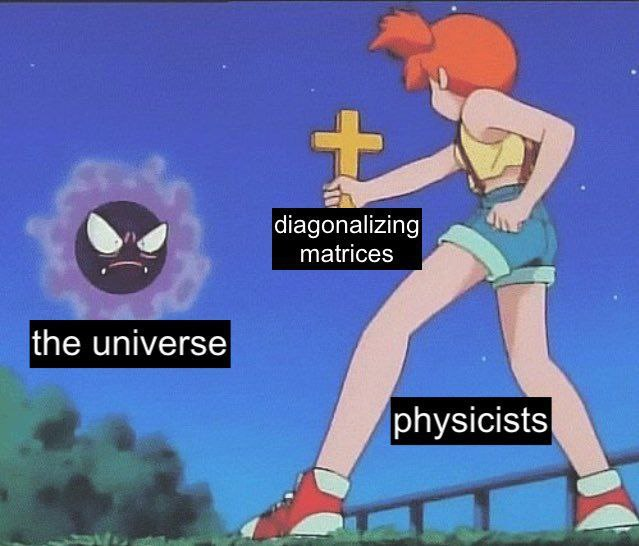
\includegraphics[]{Images/diagonalize.jpg}}The CKM matrix is what is left over when moving from one basis to another and it is the source of \textbf{flavour mixing}. The
particular matrices that cannot be simultaneously diagonalized are the $W$ boson couplings, the masses of the $d$-type quarks and the masses of the $u$-type quarks. At most it is possible to diagonalize two of these and we chose to diagonalize the masses and leave the $W$ coupling non-diagonal. It is
important to emphasize that this is a totally arbitrary choice that we are free to make. The non-trivial quark interactions come form the Yukawa sector:
\[
\pazocal{L}_{\text{Yuk}}=\overline{Q}_L^i(Y_u)^{ij}H^cu_R^j+\overline{Q}_L^i(Y_d)^{ij}Hd_r^j+\overline{l}_L^i(Y_e)^{ij}He_R^j+\text{h.c}
\]
The Higgs vacuum expectation value (vev) $v$ turns these into mass matrices, giving mass terms of the form:
\[
\pazocal{L}_{\text{mass}}=m_{ij}^d\overline{d}_L^id_R^j+m_{ij}^u\overline{u}_L^iu_R^j
\]
where the mass terms are related to the Yukawa and to the Higgs vev by:
\[
m_{ij}^q=\frac{v}{\sqrt{2}}(Y_q)^{ij}
\]
These are in general \textbf{not diagonal} and contain unphysical parameters: to remove them we have to move to the mass basis. $m$ is an arbitrary complex matrix, to diagonalize it we perform a unitary transformation acting on the left and a unitary transformation acting on the right:
\[
\hat{m}_{ij}^q=(V_L^q)_{ik}m_{kl}^q(V_R^{q\dagger})_{lj}
\]
The notation with a hat denotes that the matrix is diagonal. $L$ and $R$ have nothing to do with left- and right-handed fermions, but one can see that the $i$ index is associated with the left-quark and the $j$ index with the right-quark. Diagonalizing $m$ rotates the left- and right-handed fields:
\[
q_L^i=(V_L^q)_{ij}q_L^{'^j} \quad q_R^i=(V_R^q)_{ij}q_R^{'^j}
\]
After these transformations, the off-diagonal entries remain only in the $W$ boson couplings term:
\[
\pazocal{L}_W=\frac{g}{\sqrt{2}}\overline{u}_Li\gamma_\mu d_LW^\mu\to\frac{g}{\sqrt{2}}\overline{u}_Li\gamma_\mu(V_{u_L}V_{d_L}^\dagger)W^\mu
\]
We are now able to identify the CKM matrix as $V=V_{u_L}V_{d_L}^\dagger$ and quickly have a look at its properties:
\begin{itemize}
    \item it is \textbf{unitary}: $V^\dagger V=VV^\dagger=\mathbb{1}$. However, sometimes it is convenient to approximate it with a non-unitary matrix.
    \item The number of physical parameters is four (3 mixing angles+1 complex phase) even though there are many possible parameterizations.
    \item The general structure is:
    \[
    V=\left(\begin{array}{ccc}
    V_{ud} & V_{us} & V_{ub} \\
    V_{cd} & V_{cs} & V_{cb} \\
    V_{td} & V_{ts} & V_{tb}
\end{array}\right)
    \]
\end{itemize}
\subsection{Parametrization of the CKM Matrix}
Given the premises, we know that $V$ must contain many unphysical parameters since each $V_{ij}$ is a complex number. It is customary to choose $V_{ud}, V_{us}, V_{cb}$ and $V_{tb}$ to be purely real while the remaining elements are complex. One standard parameterization is to use \{$\theta_{12},\theta_{23},\theta_{13}$\} for the 3 mixing angles and $\delta$ for the CP-violating phase.\marginnote{Actually there are 5 phases but 4 of them are unphysical.} It is then possible to express it in the following way:
\[
V=R_{23}(\theta_{23})\mqty(\dmat{e^{-i\delta},1,1})R_{13}(\theta_{13})\mqty(\dmat{e^{+i\delta},1,1})R_{12}(\theta_{12})
\]
The three angles and the phase are such that we have:
\[
\left\{
\begin{aligned}
&\sin\theta_{12}=0.22497\pm0.00069\quad && \sin\theta_{23}=0.04229\pm0.00057\\
&\sin\theta_{13}=0.00368\pm0.00010 \quad && \delta[^\circ]=65.9\pm2.0
\end{aligned}
\right.
\]
Notice that all the mixing angles are small and it would be nice to make an approximation that captures the essential physics. The first person to make such an approximation was Wolfenstein, who noticed that the orders of magnitude of the CKM matrix seem to follow a particular pattern:
\[
|V|\sim
\left(\begin{array}{ccc}
    1 & \lambda & \lambda^3 \\
    \lambda & 1 & \lambda^2 \\
    \lambda^3 & \lambda^2 & 1
\end{array}\right)
\]
He then chose 4 new parameters to describe the physical content of the CKM matrix: $\lambda, A, \rho, \eta$.
\[
\left\{
\begin{aligned}
&\sin\theta_{12}=\lambda\\
&\sin\theta_{23}=A\lambda^2\\
&\sin\theta_{13}e^{i\delta}=A\lambda^3(\rho+i\eta)
\end{aligned}
\right.
\]
It is now possible to express the CKM matrix in function of the new 4 parameters just defined. The beauty of the \textbf{Wolfenstein parameterization} is
that we may use it to write the CKM matrix as a Taylor expansion in $\lambda$:
\[
V_W=\left(\begin{array}{ccc}
    1-\lambda^2/2 & \lambda & A\lambda^3(\rho-i\eta) \\
    -\lambda & 1-\lambda^2/2 & A\lambda^2 \\
    A\lambda^3(1-\rho-i\eta) & -A\lambda^2 & 1
\end{array}\right)
+\pazocal{O}(\lambda^4)
\]
Looking at the factors of $\lambda$, we notice that the diagonals are of order one while the elements of the upper left $2\times2$ are the expansions in $\lambda$ of sine and cosine. In fact, it is the $2\times2$ Cabibbo matrix, which means that to the first order in $\lambda$ the first two generations do not know about the third. Moreover, complex numbers show up only in the $1-3$ and $3-1$ mixing elements.\\
The new parameters have been calculated and they turn out to be:
\[
\left\{
\begin{aligned}
&\lambda=0.22574\pm0.00084 \quad &&\rho=0.152\pm0.014\\
&A=0.826\pm0.012 \quad &&\eta=0.357\pm0.010
\end{aligned}
\right.
\]
$V$ is unitary, therefore we have that $\sum_{i=1}^3V_{id}V_{is}^*=0$ and we can construct 6 relations of this type using rows and columns. In this case, we have $V_{ud}V_{us}^*\sim\lambda$, $V_{cd}V_{cs}^*\sim\lambda$ and $V_{td}V_{ts}^*\sim\lambda^5$. We can represent this equality in the complex plane obtaining a \textbf{unitarity triangle}.
\marginnote[-2cm]{
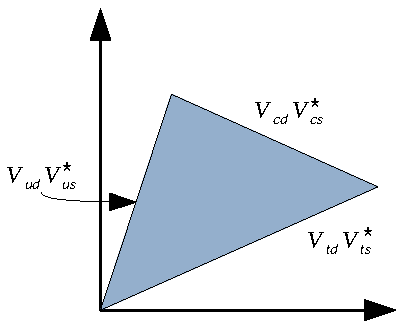
\includegraphics{Images/uni_triangle_1.pdf}
Representation of the unitarity triangle.
}
We write the 6 possible relations using all the rows and columns in the matrix, obtaining 6 different triangles which all have the same area equal to $J/2$. With this parametrization, $J$ turns out to be equal to:
\[
J=\cos\theta_{12}\cos\theta_{23}\cos^2\theta_{13}\sin\theta_{12}\sin\theta_{23}\sin\theta_{13}\sin\delta\simeq\lambda^6A^2\eta
\]
The most remarkable observation is that this quantity depends on \textit{every} physical mixing angle, therefore if \textit{any} of the mixing angle is zero there would be no CP violation. The CP violation in the SM is small but it is not small because the CP phase $\delta$ is small but it is small because of the mixing angles. We can see this in the Wolfenstein parameterization where the Jarlskog invariant comes along with six powers of $\lambda$.\\
In the example we made, the sides of the triangles are of different scaling, a better choice instead is to use $\sum_{i=1}^3V_{id}V_{ib}^*=0$ defining \textbf{the} unitarity triangle.\\
In this way, we obtain $\{V_{ud}V_{ub}^*,V_{cd}V_{cb}^*,V_{td}V_{tb}^*\}\sim\lambda^3$ and in order to have a better representation on the complex plane we can redefine everything as:
\[
\frac{V_{ud}V_{ub}^*}{V_{cd}V_{cb}^*}+1+\frac{V_{td}V_{tb}^*}{V_{cd}V_{cb}^*}=0
\]
In the picture on the side, we defined two new variables $R_u$ and $R_t$, namely:
\[
R_u=\left|\frac{V_{ud}V_{ub}^*}{V_{cd}V_{cb}^*}\right| \quad R_t=\left|\frac{V_{td}V_{tb}^*}{V_{cd}V_{cb}^*}\right|
\]
The good thing about the unitary triangle is that because each side is of $\pazocal{O}(1)$ relative to the others it is robust against experimental errors.\\
Experimentally, what are measured are the angles $(\alpha,\beta,\gamma)$ in order to obtain $(\rho,\eta)$. Moreover, the measures give us a check of consistency: if we find a strip of measurements out of the expected zone, we find an inconsistency which can be due to new physics. CP violation is present in the Standard Model but there are cosmological reasons which tell us there must be some other source of CP violation in the Universe.\marginnote[-6cm]{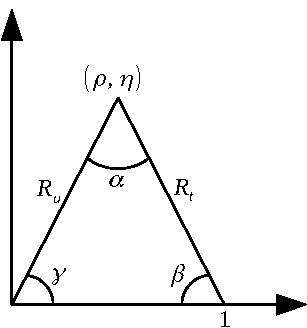
\includegraphics[]{Images/uni_triangle_2.pdf}\\
Unitarity triangle after the redefinition. The notation may vary: in California there is $(\gamma, \alpha, \beta)$ while in Japan they call them $(\phi_3,\phi_2,\phi_1)$.}
% \begin{figure}[h]
%     \centering
%     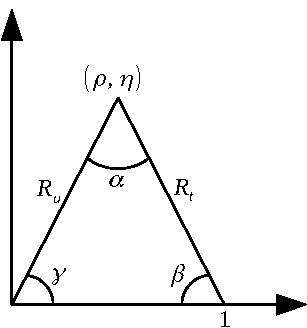
\includegraphics[width=0.4\textwidth]{Images/uni_triangle_2.pdf}
%     \caption{Unitarity triangle after the redefinition. The notation may vary: in California there is $(\gamma, \alpha, \beta)$ while in Japan they call them $(\phi_3,\phi_2,\phi_1)$.}
%     \label{fig:my_label}
% \end{figure}
\section{Flavour Changing Neutral Currents (FCNC)}\marginnote{From \cite{GT}, Section 4.}
We have chosen a basis for the quarks where the off-diagonal entries come from the $W$ boson, which we know it is charged. Therefore, the neutral boson interactions are flavour conserving.\\
Let's look at this from the experimental side and suppose we know nothing about the Standard Model, all we know are the experiments whose data are summarized in the PDG\cite{pdg}.
\begin{table}[h]
    \centering
    \begin{tabular}{c|c}
    \hline
    \rowcolor{blue!30}FCCC & FCNC\\
    \hline
    Br$(K^+\xrightarrow[]{}\mu^+\nu_\mu)=64\%$ & Br $(K_L^0\xrightarrow[]{}\mu^+\mu^-)=7\times10^{-3}$\\
    $|\Delta S|=1$ & $|\Delta S|=1$\\
    $|\Delta Q|=1$ & $|\Delta Q|=0$\\
    \hline
    Br$(B^-\xrightarrow[]{}D^0l\nu)=2.3\%$ & Br $(B^-\xrightarrow[]{}K^{*-}l^+l^-)=5\times10^{-7}$\\
    $|\Delta B|=1$ & $|\Delta B|=1$\\
    $|\Delta Q|=1$ & $|\Delta Q|=0$\\
    \hline
    \end{tabular}
    \caption{Brief summary of Flavour Changing Charged Current (FCCC) and Flavour Changing Neutral Current (FCNC) processes.}
    \labtab{fcnc}
\end{table}
\newline
Because the left-hand side of each decay is hadronic and the right-hand side is leptonic, we can determine that the processes on the left have a charged intermediate state (\textbf{charged current}) while the ones on the right have a neutral intermediate state (\textbf{neutral current}).\\
Both processes change flavour but the charged current flavour changing process proceeds at a much larger rate. One would expect both processes to come from some flavour-violating structure so that they should be of the same order of magnitude. The charged current interaction is much larger than the neutral current and this pattern only shows up in flavour-changing processes. For the flavor-conserving processes, the weak interaction charged and neutral currents indeed occur at roughly the same rates.
\subsection{FCNC at Tree-Level}
We know that the charged current, i.e. the one mediated by the $W$ boson, can change fermion flavours. How about flavour changing neutral currents (FCNC)? Let's start our discussion at tree-level. The relevant SM bosons are the photon $\gamma$, the gluon $g$, the Higgs $h$ and the $Z$ boson: \textit{why do these particles not have any tree-level FCNC?}\\
\begin{kaobox}[frametitle=Remark]
Flavour changing effects occur due to off-diagonal couplings, hence one might be tempted to say that couplings do not change flavour if they are diagonal. This is in general \underline{not true} since \textit{diagonal} is a basis dependent property. Only a \textbf{universal} matrix, i.e. one proportional to the identity, is diagonal in every basis.
\end{kaobox}
Photons and gluons cannot give FCNC at tree-level because of \textbf{gauge invariance}. Gauge symmetry forces the kinetic terms, where the gauge couplings live, to be universal. All the down-type quarks will have the same gauge interactions and as long as QCD and QED are unbroken photons and gluons are safe from tree-level FCNCs.\\
The Higgs $h$ is "accidentally" alone: how can it be flavour conserving? It couples to fermions via the Yukawa term, take for example the up-type: 
\[
(Y^u)_{ij}H^c\overline{Q}_L^iu^j+\text{h.c.}
\]
Expand $H$ around its vev, which in the unitary gauge means to consider:
\[
H=\left(\begin{array}{c}
    \frac{v+h}{\sqrt{2}} \\
    0
\end{array}\right)
\quad
\Tilde{H}=\left(\begin{array}{c}
    0\\
    \frac{v+h}{\sqrt{2}}
\end{array}\right)
\]
For the mass term we have $(m_u)_{ij}=(Y_u)_{ij}\frac{v}{\sqrt{2}}$, while for the coupling we obtain $(Y_u)_{ij}=\frac{(Y_u)_{ij}}{\sqrt{2}}$. Now we move to a basis in which the mass is diagonal:
\[
\left\{
\begin{aligned}
&u_L=V_L^uu_L'\\
&u_R=V_R^uu_R'
\end{aligned}
\right.
\Rightarrow
\left\{
\begin{aligned}
&\hat{m}_u=V_L^um_uV_R^u\\
&\hat{Y}_u=V_L^uY_u(V_R^u)^\dagger
\end{aligned}
\right.
\]
Diagonalizing the mass matrix simultaneously diagonalize the coupling. This is one example when it is sufficient for a matrix to be diagonal in the mass basis but not universal, the absence of FCNC at tree-level is due to the fact that there is only one Higgs in the SM.
\begin{kaobox}[frametitle=Two Higgs doublet model]
When looking for new physics we can \textit{either} add non-renormalizable operators \textit{or} add another Higgs.\\
We now proceed following the first idea, taking the usual Lagrangian and adding an extra-term:
\[
C_{ij}\frac{\Tilde{H}Q_L^iu_R^jH^\dagger H}{\Lambda^2}+(Y^u)_{ij}\Tilde{H}\overline{Q}_L^iu^j+\text{h.c.}
\]
This modifies both the mass and the coupling:
\[
\left\{
\begin{aligned}
&m_u=Y^u\frac{v}{\sqrt{2}}+C\left(\frac{v}{\sqrt{2}}\right)^3\frac{1}{\Lambda^2}\\
&Y_u=\frac{Y^u}{\sqrt{2}}+C\left(\frac{v}{\sqrt{2}}\right)^2\frac{1}{\Lambda^2}3\xleftarrow[]{}\text{possible combinations}
\end{aligned}
\right.
\]
If we try to diagonalize it as before, for the mass we obtain the same result while for the interaction we get:
\[
Y_h=V_L^u\left(\frac{Y^u}{\sqrt{2}}+C\frac{v^2}{2\Lambda^2}\right)(V_R^u)^\dagger+2V_L^uC\frac{v^2}{2\Lambda^2}(V_R^u)^\dagger
\]
This is not diagonal: non-renormalizable operators can give rise to FCNC at tree-level. $C_{ij}\xrightarrow[]{}(Y^u)_{ij}$ apparently cures the problem of flavour violation since $m_u\propto Y_u$ and $Y_h\propto Y_u$.\\
Now we explore the possibility of adding a second Higgs to the SM and see what happens. \marginnote{Models with two Higgs fields are important since the minimal supersymmetric models require at least two Higgs fields.}
\[
\left\{
\begin{aligned}
&H_1\sim(1,2,1/2) \quad &&\Tilde{H}_1=i\sigma_2H_1^*\\
&H_2\sim(1,2,1/2) \quad &&\Tilde{H}_2=i\sigma_2H_2^*
\end{aligned}
\right.
\]
The potential $V(H)$ gets modified into $V(H_1,H_2)$, with the most general vev pattern give by:
\[
\langle H_1 \rangle=\left(\begin{array}{c}
     0 \\
     \frac{v_1}{\sqrt{2}}
\end{array}\right)
\quad
\langle H_2 \rangle=\left(\begin{array}{c}
     W^+ \\
     \frac{v_2}{\sqrt{2}}
\end{array}\right)
\]
The parameters $v_1, v_2$ and $W^+$ are functions of the potential $V$. Since it is designed to allow U$(1)_{\text{Q}}$ symmetry, then it must be $W^+=0$. We can now count the degrees of freedom of a model with two complex SU(2) doublets, in an attempt to understand what are the fields which arise. Two complex doublets gives 4+4=8 degrees of freedom. The initial symmetry SU$(2)_{\text{L}}\times$U$(1)_{\text{Y}}$ is broken into U$(1)_{\text{Q}}$: this means that we have $2^2-1=3$ broken generators, corresponding to 3 NGBs.
\[
\text{\# degrees of freedom}=8=\underset{\mathclap{\tikz \node {$\uparrow$} node [below=1ex] {\footnotesize $H_1$ };}}{4}+\overset{\mathclap{\tikz \node {$\downarrow$} node [above=1ex] {\footnotesize $H_2$};}}{4}=\underset{\mathclap{\tikz \node {$\uparrow$} node [below=1ex] {\footnotesize  NGB};}}{3}+5=3+\underset{\mathclap{\tikz \node {$\uparrow$} node [below=1ex] {\footnotesize charged Higgs };}}{2}+\overset{\mathclap{\tikz \node {$\downarrow$} node [above=1ex] {\footnotesize neutral Higgs };}}3
\]
It is possible to assign to the neutral Higgs a CP parity, with 2 of them being even and 1 odd. The usual Higgs boson $h$ is the lightest CP even state. The generic Higgs field is given by:
\[
H_i=\left(\begin{array}{c}
    \phi_i^+\\
    \phi_i
\end{array}\right)
\underset{\mathclap{\tikz \node {$\uparrow$} node [below=1ex] {\footnotesize expand it around the v.e.v. };}}{\simeq}
\left(\begin{array}{c}
    \phi_i^+\\
    \frac{v_i+\rho_i+i\eta_i}{\sqrt{2}}
\end{array}\right)
\quad
i=1,2
\]
Guided by charge and CP parity, we can find the remaining 5 degrees of freedom.
\[
\left\{
\begin{aligned}
&(\phi_1^+,\phi_2^+)\\
&\eta_i\xrightarrow[]{}(G^0,A)\\
&\rho_i\xrightarrow[]{}(h,H)
\end{aligned}
\right.
\]
where $G^\pm$ are the two NGBs eaten by $W_L^\pm$, $H^\pm$ are the two charged Higgs fields, $G^0$ is the NGB eaten by $Z_L^0$. $A, \eta_i$ and $\rho_i$ are all neutral, with $A$ being CP odd and $\eta_i, \rho_i$ CP even. $h$ denotes the usual Higgs field and $H$ the new heavy Higgs field.\\
$\phi_i^+$ has charge equals to $\pm1$, hence we have terms like $m_{11}\phi_1^+\phi_1+m_{12}\phi_1^+\phi_2$ but not something like $\phi_1^+\rho$: we can only mix particles with the same symmetry. Now we bring our attention to the two new Higgs, $h$ and $H$:
\[
\left\{
\begin{aligned}
&\rho_1=\cos\alpha h+\sin\alpha H\\
&\rho_2=-\sin\alpha h+\cos\alpha H
\end{aligned}
\right.
\]
The parameter $\alpha$ depends on the structure of $V(H_1,H_2)$.\\
We can prove the existence of FCNC with 2 Higgs fields by doing the following exercise:
\begin{itemize}
    \item Write the most general $\pazocal{L}_{\text{Yuk}}$ including $H_1$ and $H_2$:
    \begin{align*}
    &-(Y_u^1)_{ij}\overline{Q}_L^iu_R^j\Tilde{H}_1-(Y_u^2)_{ij}\overline{Q}_L^iu_R^j\Tilde{H}_2+\text{h.c.}\\
    &-(Y_d^1)_{ij}\overline{Q}_L^id_R^jH_1-(Y_d^2)_{ij}\overline{Q}_L^id_R^jH_2+\text{h.c.}
    \end{align*}
    \item Move to the unitary gauge:
    \[
    H_i=\left(\begin{array}{c}
    \phi_i^+\\
    \frac{v_i+\rho_i+i\eta_i}{\sqrt{2}}
    \end{array}\right)
    \xrightarrow[]{}
    \left(\begin{array}{c}
    0\\
    \frac{v_i+\rho_i}{\sqrt{2}}
    \end{array}\right)
    \]
    here $v_i$ is the mass term and $\rho_i$ is proportional to the Higgs.\marginnote{We do not consider the heavy field $H$.}
    \item Compute the mass matrix and the couplings:
    \[
    \left\{
    \begin{aligned}
    &(m_u)_{ij}=\frac{1}{\sqrt{2}}\left[(Y_u^1)_{ij}v_1+(Y_u^2)_{ij}v_2\right]\\
    &(Y_h^u)_{ij}=\frac{1}{\sqrt{2}}\left[(Y_u^1)_{ij}\cos\alpha+(Y_u^2)_{ij}(-\sin\alpha)\right]
    \end{aligned}
    \right.
    \]
\end{itemize}
By introducing $u_L=V_Lu_L'$ and $u_R=V_Ru_R'$ we obtain:
\[
\pazocal{L}_{\text{Yuk}}\supset-\frac{1}{\sqrt{2}}u_L'(V_L^\dagger m_uV_R)u_R'-\frac{1}{\sqrt{2}}u_L'h(V_L^\dagger Y_hV_R)u_R'
\]
The mass term gets diagonalized, however $Y_h$ does not get diagonalized and we can have interactions like the one depicted on the side.\marginnote[-2cm]{\centering
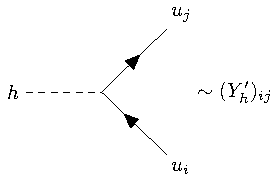
\includegraphics{Images/Yh.pdf}
\labfig{Yh}}
% \begin{figure}[h]
%     \centering
%     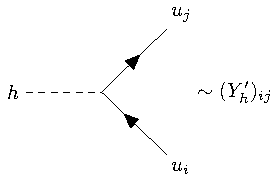
\includegraphics[width=0.45\textwidth]{Images/Yh.pdf}
%     \caption*{}
%     \labfig{Yh}
% \end{figure}
% \newline
The 2 Higgs model is important since we have two Higgs also in the SUSY model: one Higgs couples only to up quarks $(\Tilde{H}_1\to H_u)$ and one couples only to down quarks $(H_2\to H_d)$.
\[
\pazocal{L}_{\text{Yuk}}=-(Y_u)_{ij}\overline{Q}_L^iu_R^jH_u+\text{h.c}-(Y_d)_{ij}\overline{Q}_L^id_R^jH_d+\text{h.c.}
\]
With this assumption, we removed two couplings. Here interactions and mass re-align, giving us no flavour violation. The realignment of mass and interaction is always present in the SM with 1 Higgs.
\end{kaobox}
How about the $Z$? It is a gauge boson but a gauge boson of a \textit{broken} gauge symmetry so there is no reason to expect gauge invariance to protect against FCNCs. Since there are no tree-level FCNCs in the SM, we then expect to be something else protecting the $Z$.\\
It is neutral so it only connects fermions with the same charge and colour. Colour is trivially satisfied since SU$(3)_{\text{C}}$ has nothing to do with SU$(2)_{\text{L}}\times$U$(1)_{\text{Y}}$, on the other hand the electric charge is related to SU$(2)_{\text{L}}\times$U$(1)_{\text{Y}}$ by $Q=T_3+Y$. In the SM, all quarks with the same $Q$ also have the same $T_3$ and therefore the same $Y$. Recall that the $Z$ coupling only depends on these quantities:
\[
g_Z^f=g\cos\theta_wT_3-g'\sin\theta_wY
\]
Hence, particles of the same charge all have the same coupling to the $Z$, in other words the $Z$ coupling is universal for each of the up-type and, separately, down-type quarks. This is why the Standard Model $Z$ boson does not give FCNCs.
\begin{kaobox}[frametitle=Toy model]
Consider now the following toy model:
\begin{enumerate}
    \item Group symmetry: G=G$_{\text{SM}}$
    \item Fields content: 
    \[
    \left\{
    \begin{aligned}
    &Q_L\sim(3,2,+1/6) \quad &&s_L\sim(3,1,-1/3)\\
    &u_R\sim(3,1,+2/3) \quad &&s_R,d_R\sim(3,1,-1/3)\\
    &H\sim(1,2,+1/2)
    \end{aligned}
    \right.
    \]
    \item Most general Lagrangian in the Yukawa sector (for the other sectors it is just the covariant derivative):
    \begin{align*}
    \pazocal{L}_{\text{Yuk}}=-&\left[Y_u\overline{Q}_L\Tilde{H}u_R+Y_d\overline{Q}_Ld_RH+Y_s\overline{Q}_L\Tilde{H}s_R\right.\\
    &\left.+m_s\overline{s}_Ls_R+m_d\overline{s}_Ld_r+\text{h.c.}\right]
    \end{align*}
\end{enumerate}
G has dimension 7=1+6 and gets broken into H=U$(1)_{\text{B}}$ which has dimension 1. We have 10 naive parameters, corresponding to 5 moduli+5 phases:
\[
\text{\#physical parameters}=\text{\#naive}-\text{\#broken}=10-6=\underset{\mathclap{\tikz \node {$\uparrow$} node [below=1ex] {\footnotesize moduli };}}{5}+\overset{\mathclap{\tikz \node {$\downarrow$} node [above=1ex] {\footnotesize  phases};}}{5}-\underset{\mathclap{\tikz \node {$\uparrow$} node [below=1ex] {\footnotesize modulus};}}{1}-\overset{\mathclap{\tikz \node {$\downarrow$} node [above=1ex] {\footnotesize phases };}}{5}=4
\]
By removing all the phases, we obtained CP invariance. With a rotation inside U(2) we remove another parameter: $\overline{s}_L(m_ss_R+m_dd_R)=m_s\overline{s}_Ls_R$. We are now interested in diagonalizing the mass term:\marginnote{In the matrix $M$ there should have been $m_d$ instead of 0 but we killed it with the U(2) rotation.}
\[
\pazocal{L}_{\text{mass}}=-\underset{\mathclap{\tikz \node {$\uparrow$} node [below=1ex] {\footnotesize  $\frac{Y_uv}{\sqrt{2}}$};}}{m_u}\overline{u}_Lu_R-\left(\begin{array}{cc}
    \overline{d}_L & \overline{s}_L
\end{array}\right)
\underbrace{\left(\begin{array}{cc}
    \frac{Y_dv}{\sqrt{2}} & \frac{Y_sv}{\sqrt{2}} \\
    0 & m_s
\end{array}\right)}_{M}
\left(\begin{array}{c}
    d_R\\
    s_R
\end{array}\right)
\]
We can diagonalize the mass matrix through:
\[
\left(\begin{array}{c}
     d_R\\
     s_R
\end{array}\right)=V_R^\dagger\left(\begin{array}{c}
     d_R'\\
     s_R'
\end{array}\right)
\quad
\left(\begin{array}{c}
     d_L\\
     s_L
\end{array}\right)=V_L^\dagger\left(\begin{array}{c}
     d_L'\\
     s_L'
\end{array}\right)
\]
At this point, we look at the kinetic term:
\begin{align*}
\pazocal{L}_{\text{kin}}&\supset Z_\mu\sum_f\overline{f}i\gamma^\mu fg_f\\
&\supset\left(\begin{array}{c}
    \overline{d}_{L/R}' \\ \overline{s}_{L/R}'
\end{array}\right)V_{L/R}
\left(\begin{array}{cc}
    g_Z^{d_{L/R}} & 0 \\
    0 & g_Z^{s_{L/R}}
\end{array}\right)(i\gamma^\mu Z_\mu)V_{L/R}^\dagger
\left(\begin{array}{c}
    d_{L/R}' \\
    s_{L/R}' 
\end{array}\right)
\end{align*}
The couplings are given by $g_f=g\cos\theta_wT^3-g'\sin\theta_wY$, hence what we obtain is:
\[
\left\{
\begin{aligned}
&g_Z^{d_R}=g_Z^{s_R}=g\cos\theta_W\cdot0-g'\sin\theta_W(-1/3)\\
&g_Z^{d_L}=g\cos\theta_W(-1/2)-g'\sin\theta_W(-1/6)\\
&g_Z^{s_L}=g\cos\theta_W\cdot0-g'\sin\theta_W(-1/3)
\end{aligned}
\right.
\]
The crucial point is that the couplings in the right sector are identical, i.e.: 
\[
V_R\left(\begin{array}{cc}
    g_Z^{d_R} & 0 \\
    0 & g_Z^{s_R}
\end{array}\right)V_R^\dagger\sim\mathbb{1}g_Z^{d_R}
\]
Therefore we have no flavour violation. In the left sector instead we parametrize $V_L$ as:
\[
V_L=\left(\begin{array}{cc}
    \cos\theta & \sin\theta \\
    -\sin\theta & \cos\theta
\end{array}\right)
\]
so that we find:
\[
V_L\left(\begin{array}{cc}
    g_Z^{d_L} & 0 \\
    0 & g_Z^{s_L}
\end{array}\right)V_L^\dagger=\left(\begin{array}{cc}
    g_Z^{d_L}c^2 _\theta+g_Z^{s_L}s^2 _\theta & (g_Z^{d_L}-g_Z^{s_L})c _\theta s _\theta \\
    (g_Z^{d_L}-g_Z^{s_L})c _\theta s _\theta & g_Z^{d_L}s^2 _\theta+g_Z^{s_L}c^2 _\theta
\end{array}\right)\marginnote{$c_\theta=\cos\theta$ and $s_\theta=\sin\theta$.}
\]
The flavour violation is given by the terms proportional to $(g_Z^{d_L}-g_Z^{s_L})$.\marginnote{\centering
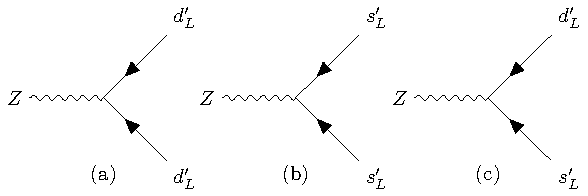
\includegraphics{Images/feynmanabc.pdf}
\labfig{feynmanabc}}
% \begin{figure}[h]
%     \centering
%     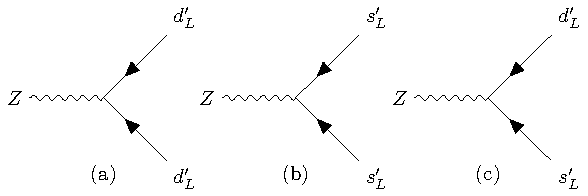
\includegraphics{Images/feynmanabc.pdf}
%     \caption*{}
%     \labfig{feynmanabc}
% \end{figure}
Diagram (a) refers to $g_Z^{d_L}\cos^2\theta+g_Z^{s_L}\sin^2\theta$, (b) to $g_Z^{d_L}\sin^2\theta+g_Z^{s_L}\cos^2\theta$ and the flavour violating one (c) to $(g_Z^{d_L}-g_Z^{s_L})\cos\theta\sin\theta$.\\
% In fact, in our toy model we have:
% \begin{table}[h]
%     \centering
%     \begin{tabular}{c|cc}
%     \hline
%      & G & H \\
%      \hline
%      Right sector & $\begin{cases}
%      d_R\sim(3,1,-1/3)\\
%      s_R\sim(3,1,-1/3)
%      \end{cases}$ & $(3,-1/3)$\\
%      \hline
%      Left sector & $\begin{cases}
%      d_L\sim(3,2,1/6)\\
%      s_L\sim(3,1,-1/3)
%      \end{cases}$ & $(3,-1/3)$\\
%      \hline
%     \end{tabular}
%     \caption{No flavour violation in the right sector, flavour violation in the left sector.}
%     \label{tab:my_label}
% \end{table}\\
In the SM, there is no flavour violation because $g_Z^{d_L}=g_Z^{s_L}$. The left sector is a quark doublet (3,2,1/6) while in this toy model we have $s_L$ and $d_L$ coming from different irreps of the unbroken group.
\end{kaobox}
\subsection{FCNC at Loop-Level}\marginnote{From \cite{GT}, Section 5.}
So far, we studied everything at tree-level. In the mass basis, the $W$ changes flavour while the other bosons do not, pretty simple. As it is often the case, the story is more subtle at loop-level. Loop-level contributions are usually small compared to the tree-level diagrams for the same process. A loop correction to a tree-level process is hard to observe, while a small effect which is the only source of signal has at least a chance of being measured well. A
natural set of processes to look at are those that generate FCNCs, since we already know that these vanish at tree-level in the Standard Model.\\
The Glashow-Iliopoulos-Maiani (GIM) mechanism is the mechanism through which FCNCs are suppressed in loop diagrams. The underlying principle is that for a unitary matrix, any pair of columns (or rows) are orthogonal. The first non-trivial point is that
loop-level FCNCs are most sensitive to the heavy quarks running in the loops, so that we can be sensitive to the top. As an example, we study the process $s\to de^+e^-$, which is represented at one-loop by the following diagram.\\
\begin{figure}[h]
    \centering
    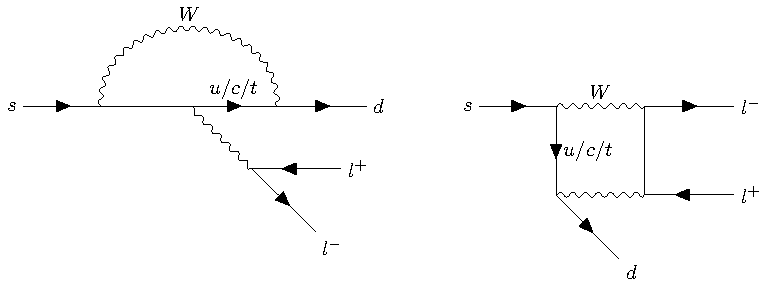
\includegraphics{Images/gim.pdf}
    \caption*{}
    \labfig{gim}
\end{figure}\\
\newline
The amplitude is proportional to the CKM matrix, in particular:
\[
\pazocal{M}\propto\sum_{i=u,c,t}V_{is}^*f(m_i)V_{id}=\sum_{i=u,c,t}(V^\dagger)_{si}\Tilde{f}(x_i)V_{id}
\]
where $x_i=m_i^2/m_W^2$ and $\Tilde{f}(x_i)$ is the Inami-Lim function.\\
When the GIM mechanism was proposed, there were only three quarks (up, down and strange). However, it required the existence of a \textbf{fourth quark}, the charm: the introduction of the fourth quark restored unitarity of the flavour mixing matrix, allowing to drop constant terms in $\Tilde{f}$. How? If $\Tilde{f}=$ constant, then we have $\sum_{i=u,c,t}=(V^\dagger)_{si}V_{id}=\delta_{sd}=0$. This gives us a non-trivial information about the quarks running in the loop. Suppose to have only two families, the CKM matrix becomes:
\[
V=\left(\begin{array}{cc}
    \cos\theta_c & \sin\theta_c \\
    -\sin\theta_c & \cos\theta_c
\end{array}\right)
\]
In the loop we have $(m_{u/c}/m_W)^2\ll1$, so it is possible to expand $\Tilde{f}$ and compute the amplitude:
\[
\left\{
\begin{aligned}
&\Tilde{f}(x)=\cancelto{\text{constant}}{\Tilde{f}(0)}+\Tilde{f}'(0)x+\pazocal{O}(x^2)\\
&\pazocal{M}\propto V_{us}^*V_{ud}\frac{m_u^2}{m_W^2}+V_{cs}^*V_{cd}\frac{m_c^2}{m_W^2}=\cos\theta_c\sin\theta_c\left(\frac{m_c^2-m_u^2}{m_W^2}\right)
\end{aligned}
\right.
\]
If $m_u=m_c$, the contribution of the diagram with the up quark running in the loop would be perfectly canceled by the one with the charm quark running in the loop. The amplitude can be expressed as a function of $m_u/m_c$ and it is something which goes like:
\[
\pazocal{M}\sim\frac{m_c^2}{m_W^2}\left(1-\frac{m_u^2}{m_c^2}\right)
\]
The term between parentheses is much closer to zero than it is to one but it is multiplied by a very small factor. In fact, the GIM mechanism tells us that the neutral current process is suppressed by a loop factor \textit{and} by a GIM factor:
\[
\pazocal{M}\sim\frac{g^2}{16\pi^2}\frac{m_c^2}{m_W^2}
\]
The calculations from Gaillard and T.D. Lee gave a prediction for the mass of the charm quark of $m_c=1.5$\,GeV which is remarkably close. It turns out that they had luck on their side, since if one follows their calculation more honestly, one obtains a value between 0.5 and 10. The charm was finally observed in 1974 at SLAC and Brookhaven. Which quarks dominate the mixing? By comparing the loops with an internal top and charm we get:
\[
\pazocal{M}_t\propto\underset{\mathclap{\tikz \node {$\uparrow$} node [below=1ex] {\footnotesize  $\pazocal{O}(1)$};}}{\frac{m_t^2}{m_W^2}}\overset{\mathclap{\tikz \node {$\downarrow$} node [above=1ex] {\footnotesize $\sim\lambda^5$};}}{V_{td}V_{ts}^*} \quad \pazocal{M}_c\propto\underset{\mathclap{\tikz \node {$\uparrow$} node [below=1ex] {\footnotesize  $\sim(10^{-2})^2$};}}{\frac{m_c^2}{m_W^2}}\overset{\mathclap{\tikz \node {$\downarrow$} node [above=1ex] {\footnotesize $\sim\lambda$};}}{V_{cd}V_{cs}^*}
\]
It turns out that the charm wins, so in this sense Gaillard and Lee got lucky once again since back then nobody would have believed that the top was so heavy that it might challenge the charm contribution.
\section{Running of the Strong Coupling Constant}
What we want to do is to renormalize divergencies in QFT, hence we use \textbf{dimensional regularization}. As seen in \refch{intro}, we know that in terms of energy $\left[\int d^Dx\pazocal{L}(x)\right]=0$, therefore $\left[\pazocal{L}\right]=D=4-2\varepsilon$. This implies that the terms $\partial^\mu\phi\partial_\mu\phi$, $\overline{\Psi}\slashed{\partial}\Psi$ and $g\overline{\Psi}\slashed{A}\Psi$ must all have dimension $D$:
\[
\left[\phi\right]=1-\varepsilon \quad \left[\Psi\right]=\frac{3}{2}-\varepsilon \quad \left[g\right]=\varepsilon\xleftarrow[]{}\text{no good \raisebox{-\mydepth}{{
\includegraphics[height=1.1\baselineskip]{Images/sadsmile.jpg}}}}
\]
The gauge coupling constant acquires dimensions! This is a prelude to the non-trivial behaviour of the renormalized coupling constant as a function of the energy scale.\marginnote{From \cite{introQCD}, Section 3.} Before we come to that, let's write the bare Lagrangian of QCD, assuming for the moment that all the fields are massless:\marginnote{The assumption of massless fields is called \textbf{chiral limit}.}
\[
\pazocal{L}_0=\overline{\Psi}_Bi\slashed{\partial}\Psi_B-\frac{1}{4}F_{\mu\nu,B}^aF^{\mu\nu,a}_B+g_B\overline{\Psi}_B\slashed{A}_B\Psi_B+\text{(gauge fixing terms, ghosts)}
\]
The bare fields can be expressed in terms of the renormalized ones via the renormalization constants, which are all dimensionless:
\[
\Psi_B=Z_2^{1/2}\Psi_R \quad A^\mu_B=Z_3^{1/2}A^\mu_R \quad g_B=Z_g\mu^\varepsilon g_R
\]
Here, $[g_R]=0$ and the dimensionality is put into the parameter $\mu$. The terms present in the Lagrangian can now be written as follows:
\[
Z_2\overline{\Psi}_Ri\slashed{\partial}\Psi_R=\overline{\Psi}_Ri\slashed{\partial}\Psi_R+(Z_2-1)\overline{\Psi}_Ri\slashed{\partial}\Psi_R=\overline{\Psi}_Ri\slashed{\partial}\Psi_R+\delta_2\overline{\Psi}_Ri\slashed{\partial}\Psi_R
\]
We do the same for $F_{\mu\nu}F^{\mu\nu}$ obtaining $\delta_3=Z_3-1$, while for the last term we get:
\[
g_B\overline{\Psi}_B\slashed{A}_B\Psi_B=Z_gZ_2Z_3^{1/2}\overline{\Psi}_R\slashed{A}_R\Psi_Rg_R\mu^\varepsilon
\]
It is customary to define $Z_1$ as:
\[
Z_1=Z_gZ_2Z_3^{1/2}=1+Z_1-1=1+\delta_1
\]
How do we compute these counter terms which cancel the divergencies? $\delta_2$ is obtained from quark self-energy, while gluon self-energy gives $\delta_3$. The $q\overline{q}g$ vertex corrections gives us $\delta_1$.\marginnote{
Quark self-energy:\\
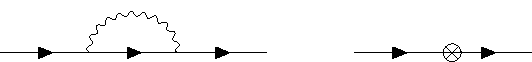
\includegraphics{Images/delta2.pdf}\\
Gluon self-energy:\\      
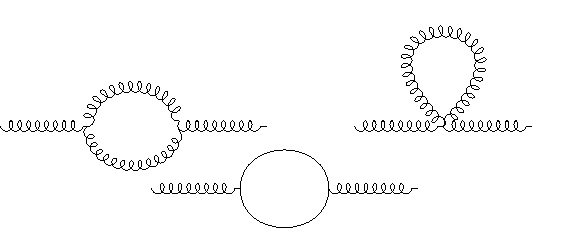
\includegraphics{Images/delta3.pdf}\\
$q\overline{q}g$ vertex corrections:\\
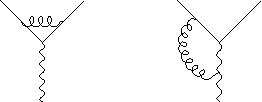
\includegraphics{Images/delta1.pdf}
}
% \begin{figure}[h]
%     \centering    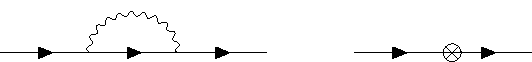
\includegraphics{Images/delta2.pdf}
%     \caption*{}
%     \labfig{delta2}
% \end{figure}\\
% \newline
% \newline
% $\delta_3$ is obtained from the gluon self-energy:\\
% \begin{figure}[h]
%     \centering
%     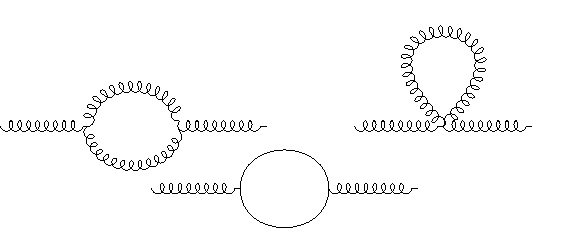
\includegraphics{Images/delta3.pdf}
%     \caption*{}
%     \labfig{delta3}
% \end{figure}\\
% For $\delta_1$ we have to consider $\overline{q}qg$ vertex corrections:\\
% \begin{figure}[h]
%     \centering
%     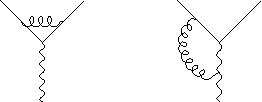
\includegraphics[width=0.45\textwidth]{Images/delta1.pdf}
%     \caption*{}
%     \labfig{delta1}
% \end{figure}\\
Summarizing, we get:
\[
\left\{
\begin{aligned}
&\text{quark self-energy:}&&\delta_2=-C_F\frac{\alpha_s}{4\pi\varepsilon}\\
&\text{gluon self-energy:}&&\delta_3=\left(\frac{5}{3}C_A-\frac{4}{3}n_fT_F\right)\frac{\alpha_s}{4\pi\varepsilon}\\
&\text{$\overline{q}qg$ vertex corrections:}&&\delta_1=-(C_A+C_F)\frac{\alpha_s}{4\pi\varepsilon}
\end{aligned}
\right.
\]
where $\alpha_s=g_R^2/4\pi$, $C_F$ is such that $C_FN=\Tr{\sum_a\lambda^a\lambda^a}=(N^2-1)/2$ for SU(N), $C_A=N$, $n_f$ denotes the number of flavours and $T_F$ is such that $\Tr{T_F^aT_F^b}=T_F\delta^{ab}$.\\
Using these results and the definition of $Z_1$ we get:
\begin{align*}
Z_g&=Z_g(\alpha_s)=\frac{Z_1}{Z_2Z_3^{1/2}}\simeq1+\delta_1-\delta_2-\frac{1}{2}\delta_3\\
&=1+\frac{\alpha_s}{4\pi\varepsilon}\left(-\frac{11}{6}C_A+\frac{2}{3}n_fT_F\right):=1-\frac{\alpha_s}{\varepsilon}\frac{b_0}{2}
\end{align*}
At this point we may ask ourselves a totally legit question: \textit{why in the heavenly name of God do we need all this terms}? The answer is that we would like to find a differential equation telling us how the renormalized coupling $g_R$ evolves with $\mu$, arriving at the end to an expression of $\alpha_s(\mu)$.\\
The starting point is to consider $\frac{d}{d\mu}g_B=0$, i.e. the bare coupling \textit{does not know} about $\mu$. The parameter $\mu$ is an artifact of the regularization prescription, introduced to define the dimensional coupling in $D$ dimensions, therefore it should not enter in measurable quantities. The bare coupling is given by $g_B=\mu^\varepsilon Z_g g_R$, so that when differentiating with respect to $\mu$ one gets:
\begin{align*}
\mu\frac{dg_B}{d\mu}=0&=\mu\left[\frac{dZ_g}{d\mu}\mu^\varepsilon g_R+\varepsilon\mu^{\varepsilon-1}Z_gg_R+Z_g\mu^\varepsilon\frac{dg_R}{d\mu}\right]\\
&=\mu^\varepsilon Z_gg_R\left[\frac{\mu}{Z_g}\frac{dZ_g}{d\mu}+\varepsilon+\frac{\mu}{g_R}\frac{dg_R}{d\mu}\right]
\end{align*}
At the leading order in $g_R$, $Z_g=1$ therefore:
\[
\mu\frac{dg_R}{d\mu}=-\varepsilon g_R
\]
Moving to the next order we have:
\[
\mu\frac{dZ_g}{d\mu}=\mu\frac{d}{d\mu}\left(1-\frac{b_0g_R^2}{8\pi\varepsilon}\right)=-\frac{b_0g_R}{4\pi\varepsilon}\mu\frac{dg_R}{d\mu}=\frac{b_0g_R^2}{4\pi}
\]
where in the last step we used the relation obtained above. Putting everything together we get:
\[
\beta(g_R):=\mu\frac{dg_R}{d\mu}=-\varepsilon g_R-\frac{b_0g_R^3}{4\pi}
\]
Translating this into a function of $\alpha_s$ results in:
\[
\beta(\alpha_s):=\mu\frac{d\alpha_s}{d\mu}=\frac{g_R}{2\pi}\mu\frac{dg_R}{d\mu}=-\frac{\varepsilon g_R^2}{2\pi}-\frac{b_0g_R^4}{8\pi^2}=-2\varepsilon\alpha_s-2b_0\alpha_s^2
\]
For $\varepsilon=0$ we can solve the differential equation given by:
\[
\mu\frac{d\alpha_s}{d\mu}=-2b_0\alpha_s^2 \quad \text{with}\,b_0\stackrel{N=3}{=}\frac{1}{12\pi}(33-2n_f)
\]
% and now we do what is called a pro gamer move: instead of differentiating with respect to $\mu$, we differentiate with respect to $\frac{d}{dt}=\mu^2\frac{d}{d\mu^2}=\frac{d}{d\ln\mu^2}$. We then get:
% \[
% \varepsilon\mu^{2\varepsilon}Z_g^2\alpha_s+2\mu^{2\varepsilon}Z_g\alpha_s\frac{dZ_g}{dt}+\mu^{2\varepsilon}Z_g^2\frac{d\alpha_s}{dt}=0
% \]
% $Z_g$ depends on $\mu$ through $\alpha_s$, we can define $\beta(\alpha_s):=\frac{d\alpha_s}{dt}$ and write the previous expression as follows:
% \begin{align*}
% &\varepsilon\alpha_s+2\frac{\alpha_s}{Z_g}\frac{dZ_g}{d\alpha_s}\frac{d\alpha_s}{dt}+\frac{d\alpha_s}{dt}=0\\
% &\varepsilon\alpha_s+2\alpha_s\left(-\frac{b_0}{2\varepsilon}\right)\beta(\alpha_s)+\beta(\alpha_s)=0\\
% &\beta(\alpha_s)=-\frac{\varepsilon\alpha_s}{1-b_0\alpha_s/\varepsilon}\simeq-\varepsilon\alpha_s\left(1+\frac{b_0\alpha_s}{\varepsilon}\right)+\pazocal{O}(\alpha_s^3)=-b_0\alpha_s^2
% \end{align*}
% In this way, we obtain a differential equation for $\alpha_s$:
% \[
% \frac{d\alpha_s}{dt}=-b_0\alpha_s^2 \quad \text{with}\,b_0\stackrel{N=3}{=}\frac{1}{12\pi}(33-2n_f)
% \]
The sign of $b_0$ tells us if we are going towards the infrared or the ultraviolet region. $b_0>0$ for $n_f<16$, which is our case since we are dealing with $n_f=6$. We can now solve this equation:
\[
\int_{\alpha(\mu)}^{\alpha(\Lambda)}\frac{d\alpha_s}{\alpha_s^2}=-2b_0\int_\mu^\Lambda\frac{d\mu'}{\mu'}
\]
where $\Lambda$ is the boundary condition of the first order differential equation and corresponds to the scale at which the coupling becomes infinity. Computing the integral gives us:
\[
\frac{1}{\alpha_s(\mu)}-\frac{1}{\alpha_s(\Lambda)}=-2b_0\ln{(\Lambda/\mu)}=b_0\ln{(\mu^2/\Lambda^2)}
\]
At 1-loop, the coupling gets smaller in the ultraviolet region and bigger in the infrared region:
\begin{equation}
\labeq{alpha_s}
\alpha_s(\mu)=\frac{1}{b_0\ln(\mu^2/\Lambda_{\text{QCD}}^2)}
\end{equation}
\marginnote[-5cm]{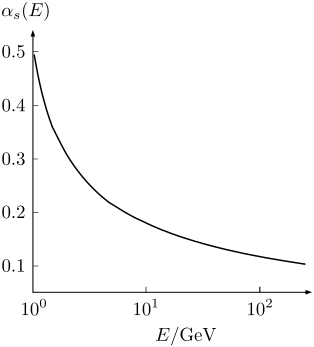
\includegraphics[]{Images/couplingconstant.png}\\
From \href{https://commons.wikimedia.org/wiki/File:Strong_coupling_as_function_of_energy.svg}{WikiMedia}: strong coupling constant as a function of energy.}
\section{Renormalization Group Invariance}
The fact that the coupling constant $\alpha_s$ depends on the unphysical renormalization scale $\mu$ should not be a source of worry since the coupling constant is \textit{not} an observable. What we observe are instead decay rates, spectra or cross sections, given by the product of the coupling constant and some matrix element. The matrix element will in general acquire a non-trivial renormalization scale dependence through the renormalization procedure, therefore we just need to check that the $\mu$ dependence of the coupling constant and of the matrix element cancel each other.
Consider now a physical observable, e.g. the ratio: 
\[
R=\frac{\sigma(e^+e^-\to\text{hadrons})}{\sigma(e^+e^-\to\mu^+\mu^-)}
\]
This will depend on the center of mass energy $s$, now we want to compute it at an energy scale far away from $\Lambda_{\text{QCD}}$. At the leading order, it is equal to $3\sum_fQ_f^2$ and we want to include QCD corrections. Neglecting the quark masses, the scales in the game are $s$ and $\mu$, giving rise to a series expansion in terms of the renormalized coupling $\alpha_s(\mu)$:
\[
R(\alpha_s(\mu),t=s/\mu^2)=1+\alpha_sf_1(t)+\alpha_s^2f_2(t)+\cdots=\sum_{n=0}^\infty\alpha_s^nf_n(t)
\]
$R$ has a clear dependence on $\alpha_s$ and on $\mu$ via the functions $f_n(t)$. Being it an observable, it should be independent on $\mu$:
\begin{align*}
0=\mu\frac{d}{d\mu}R(\alpha_s(\mu),t=s/\mu^2)=&\beta(\alpha_s)f_1(t)+\alpha_s\mu\frac{df_1(t)}{d\mu}\\
&+2\alpha_s\beta(\alpha_s)f_2(t)+\alpha_s^2\mu\frac{df_2(t)}{d\mu}+\cdots
\end{align*}
At order $\alpha_s$ we have $\mu\frac{df_1(t)}{d\mu}=0$ hence $f_1(t)=$ constant $=a_1$ and there is no dependence on $t$ (therefore on $\mu$). This is a non-trivial result, it is telling us that $R$ at 1-loop is finite and all infinities must cancel without charge renormalization. If they did not cancel, $f_1$ would depend explicitly on $\mu$: this is a consequence of the fact that colour interactions do not enter in the renormalization of the electric charge.\\
At order $\alpha_s^2$ we have:
\[
\beta(\alpha_s)a_1+\alpha_s^2\mu\frac{df_2(t)}{d\mu}=0\Rightarrow f_2(t)=a_2+b_0a_1\ln(\mu^2/s)
\]
\marginnote[-2cm]{Full calculation for $f_2(t)$:
\begin{align*}
&\beta(\alpha_s)a_1+\alpha_s^2\mu\frac{df_2(t)}{d\mu}=-2b_0\alpha_s^2a_1+\alpha_s^2\mu\frac{df_2(t)}{dt}\frac{dt}{d\mu}=\\
&-\cancel{2}b_0a_1\cancel{\alpha_s^2}-\frac{\cancel{2}s}{\mu^2}\cancel{\alpha_s^2}\frac{df_2}{dt}=-b_0a_1-t\frac{df_2(t)}{dt}=0
\end{align*}
It follows that:
\[
df_2(t)=-\frac{dt}{t}b_0a_1
\]
and the result is obtained by integrating this quantity.}
We obtained the leading log-effect at 2-loops using only 1-loop computations. So far, up to order $\alpha_s^2$ we obtained:
\[
R=1+\underbrace{a_1\alpha_s}_{\text{1-loop}}+\underbrace{b_0a_1\alpha_s^2\ln(\mu^2/s)+a_2\alpha_s^2}_{\text{2-loops}}+\pazocal{O}(\alpha_s^3)
\]
Carrying out the computations at higher orders allows us to express the generic function $f_n(t)$ as $f_n(t)=a_1[b_0\ln(\mu^2/s)]^n$. Putting all the terms together, we arrive to the following expression of the ratio $R$:
\begin{align*}
R&=1+a_1\alpha_s\left\{1+b_0\alpha_s\ln\left(\frac{\mu^2}{s}\right)+\left[b_0\alpha_s\ln\left(\frac{\mu^2}{s}\right)\right]^2+\cdots\right\}+a_2\alpha_s^2+\cdots\\
&=1+a_1\frac{\alpha_s(\mu)}{1+\alpha_s(\mu)b_0\ln(s/\mu^2)}+a_2\alpha_s^2+\cdots
\end{align*}
Moreover, keeping in mind the expression of $\alpha_s(\mu)$ we found in the previous section [\refeq{alpha_s}], the fraction above can be written as:
\begin{align*}
\frac{\alpha_s(\mu)}{1+\alpha_s(\mu)b_0\ln\left(\frac{s}{\mu^2}\right)}&=\frac{1}{b_0\ln\left(\frac{\mu^2}{\Lambda_{\text{QCD}}^2}\right)}\frac{1}{1+\frac{1}{b_0\ln(\mu^2/\Lambda_{\text{QCD}}^2)}b_0\ln\left(\frac{s}{\mu^2}\right)}\\
&=\frac{1}{b_0\ln(\mu^2/\Lambda_{\text{QCD}}^2)+b_0\ln(s/\mu^2)}\\
&=\frac{1}{b_0\ln(s/\Lambda_{\text{QCD}}^2)}=\alpha_s(s)
\end{align*}
Renormalization Group Invariance constraints the form of higher-order corrections and the higher-order logarithmic terms can be resummed by simply setting the scale of $\alpha_s$ to $s$. The final result will be in the form:
\[
R=1+a_1\alpha_s(s)+a_2\alpha_s(s)^2+a_3\alpha_s(s)^3+\cdots
\]
From $\alpha_s(m_Z)=0.118$ we can extract:
\[
\left\{
\begin{aligned}
&\Lambda_{\text{QCD}}=89.9\,\text{MeV at 1-loop with $n_f=5$}\\
&\Lambda_{\text{QCD}}=213.3\,\text{MeV at 4-loop with $n_f=5$}
\end{aligned}
\right.
\]
$\Lambda_{\text{QCD}}$ determines the separation between light and heavy quarks: below $\Lambda_{\text{QCD}}$ we have the light quarks ($u, d, s$), above we have the heavy quarks ($t, b, c$).
\section{Symmetries of QCD}\marginnote{From \cite{SS}, Section 1.3.}
\labsec{symmqcd}
The lightest meson and baryon containing a charm quark are $D^+=c\overline{d}$ and $\Lambda_c^+=udc$ with masses, respectively, of 1869.4 MeV and 2284.9 MeV. The threshold center of mass energy to produce a $D^+D^-$ pair in $e^+e^-$ collisions is approximately 3.74 GeV, way beyond the low-energy regime we are interested in. Therefore, we will approximate the full QCD Lagrangian with its light flavour version, i.e. ignoring effects due to heavy quark-antiquark pairs.\\
% By comparing the proton mass with the sum of the masses of its constituents, it is easy to see that $m_p\gg2m_u+m_d$, therefore an interpretation of the proton mass in terms of current-quark
% mass parameters must be very different from, say, the situation in the hydrogen atom, where the mass is essentially given by the sum of the electron
% and proton masses, corrected by a small amount of binding energy.\\
The QCD Lagrangian containing only light flavours in the chiral limit ($m_u,m_d,m_s\to0$) is a good starting point in the discussion of low energy QCD:\marginnote{The covariant derivative acts on colour and Dirac indices only but it is independent of flavour.}
\[
\pazocal{L}_{\text{QCD}}^0=\sum_{f=u,d,s}\overline{q}_fi\slashed{D}q_f-\frac{1}{2}\Tr{G_{\mu\nu}G^{\mu\nu}}
\]
Our goal is to analyze the symmetry of the QCD Lagrangian with respect to independent global transformations of the left- and right-handed fields. There are 16 independent $4\times4$ matrices that can be expressed in terms of the identity, $\gamma^\mu$, $\gamma_5$, $\gamma^\mu\gamma_5$ and $\sigma^{\mu\nu}=i[\gamma^\mu,\gamma^\nu]/2$. In order to decompose this 16 quadratic forms into their projection for left- and right-handed fields, we use:\marginnote{Remember that:
\[
\left\{
\begin{aligned}
&q_L=P_Lq &&q_R=P_Rq\\
&\overline{q}_L=\overline{q}P_L &&\overline{q}_R=\overline{q}P_R
\end{aligned}
\right.
\]
where the two projection operators are given by:
\[
P_L=\frac{1-\gamma_5}{2}=P_L^\dagger \qquad P_R=\frac{1+\gamma_5}{2}=P_R^\dagger
\]}
\begin{equation}
\labeq{gammarelations}
\overline{q}\Gamma_iq=\left\{
\begin{aligned}
&\overline{q}_R\Gamma_1q_R+\overline{q}_L\Gamma_1q_L \quad \text{for}\,\Gamma_1\in\{\gamma^\mu,\gamma^\mu\gamma_5\}\\
&\overline{q}_R\Gamma_2q_L+\overline{q}_L\Gamma_2q_R \quad \text{for}\,\Gamma_2\in\{\mathbb{1},\gamma_5,\sigma^{\mu\nu}\}
\end{aligned}
\right.
\end{equation}
We now apply this to the term of $\pazocal{L}_{\text{QCD}}^0$ containing the contraction of the covariant derivative with $\gamma^\mu$. This quadratic form decouples into the sum of two terms which connect left-handed with left-handed and right-handed with right-handed fields.
\[
\pazocal{L}_{\text{QCD}}^0=\sum_{f=u,d,s}(\overline{q}_{L,f}i\slashed{D}q_{L,f}+\overline{q}_{R,f}i\slashed{D}q_{R,f})-\frac{1}{2}\Tr{G_{\mu\nu}G^{\mu\nu}}
\]
Due to flavour independence of the covariant derivative, $\pazocal{L}_{\text{QCD}}^0$ is invariant under:
\[
q_{L}=\left(\begin{array}{c}
    u_{L}\\
    d_{L}\\
    s_{L}
\end{array}\right)\to U_L\left(\begin{array}{c}
    u_{L}\\
    d_{L}\\
    s_{L}
\end{array}\right)
\qquad
q_{R}=\left(\begin{array}{c}
    u_{R}\\
    d_{R}\\
    s_{R}
\end{array}\right)\to U_R\left(\begin{array}{c}
    u_{R}\\
    d_{R}\\
    s_{R}
\end{array}\right)
\]
where $U_{L}$ and $U_R$ are given by:
\begin{equation}
\labeq{transformation}
U_{L}=\exp{-i\sum_{a=1}^8\theta_a^{L}\frac{\lambda^a}{2}}e^{-i\theta_{L}}
\qquad
U_{R}=\exp{-i\sum_{a=1}^8\theta_a^{R}\frac{\lambda^a}{2}}e^{-i\theta_{R}}
\end{equation}
$U_L$ and $U_R$ are independent $3\times3$ unitary matrices. $\overline{q}_{L/R}$ transforms as $\overline{q}_{L/R}\to\overline{q}_{L/R}'U_{L/R}^\dagger$ and by performing explicit computations, one easily obtains:
\[
\overline{q}_{L/R}i\slashed{D}q_{L/R}\to\overline{q}_{L/R}U_{L/R}^\dagger U_{L/R}i\slashed{D}q_{L/R}=\overline{q}_{L/R}i\slashed{D}q_{L/R} \quad \checkmark
\]
$\pazocal{L}_{\text{QCD}}^0$ is said to have a classical global U$(3)_{\text{L}}\times$U$(3)_{\text{R}}$ symmetry. Applying N\"other's Theorem, one would expect then to have 2$\times$(8+1)=18 conserved currents.
\begin{kaobox}[frametitle=N\"other's Theorem]
N\"other's Theorem establishes the connection between continuous symmetries of a dynamical system and conserved quantities. In order to identify the conserved currents associated with the transformation of \refeq{transformation}, we shortly recall the method of Gell-Mann and Levy which will then be applied to $\pazocal{L}_{\text{QCD}}^0$. We start with a Lagrangian depending on $n$ independent fields $\phi_i$ and their partial derivatives, from which we obtain $n$ equation of motions:
\[
\pazocal{L}(\phi_i,\partial_\mu\phi_i)\to\frac{\partial\pazocal{L}}{\partial\phi_i}-\partial_\mu\frac{\partial\pazocal{L}}{\partial(\partial_\mu\phi_i)}=0 \quad i=1,\cdots,n
\]
Suppose that this Lagrangian is invariant under a global symmetry transformation depending on $r$ real parameters: the method of Gell-Mann and Levy consist of promoting this global symmetry to a local one. We consider transformations which depend on $r$ local parameters $\varepsilon_a(x)$:
\[
\phi_i(x)\to\phi_i'(x)=\phi_i(x)+\delta\phi_i(x)=\phi_i(x)-i\varepsilon_a(x)F_i^a(\phi)
\]
How does $\pazocal{L}$ react to this type of transformation? We neglect terms of order $\varepsilon^2$ and higher and obtain:
\begin{align*}
\delta\pazocal{L}=&\frac{\partial\pazocal{L}}{\partial\phi_i}\delta\phi_i+\frac{\partial\pazocal{L}}{\partial(\partial_\mu\phi_i)}{\color{blue}\partial_\mu\delta\phi_i}\\
=&\frac{\partial\pazocal{L}}{\partial\phi_i}\delta\phi_i+\frac{\partial\pazocal{L}}{\partial(\partial_\mu\phi_i)}{\color{blue}[-i\partial_\mu\varepsilon_a(x)F_i^a(\phi)-i\varepsilon_a(x)\partial_\mu F_i^a(\phi)]}\\
=&\varepsilon_a(x)\left(-i\frac{\partial\pazocal{L}}{\partial\phi_i}F_i^a(\phi)-i\frac{\partial\pazocal{L}}{\partial(\partial_\mu\phi_i)}\partial_\mu F_i^a(\phi)\right)\\
&+\partial_\mu\varepsilon_a(x)\left(-i\frac{\partial\pazocal{L}}{\partial(\partial_\mu\phi_i)}F_i^a(\phi)\right)\\
=&\varepsilon_a(x)\partial_\mu J^{\mu,a}+\partial_\mu\varepsilon_a(x)J^{\mu,a}
\end{align*}
For each infinitesimal transformation, we define a four-current density given by:
\[
J^{\mu,a}=-i\frac{\partial\pazocal{L}}{\partial(\partial_\mu\phi_i)}F_i^a(\phi) \qquad \partial_\mu J^{\mu,a}=-i\frac{\partial\pazocal{L}}{\partial\phi_i}F_i^a(\phi)-i\frac{\partial\pazocal{L}}{\partial(\partial_\mu\phi_i)}\partial_\mu F_i^a(\phi)
\]
From the expression of $\delta\pazocal{L}$, it is easy to obtain the four-currents and their divergences as:
\begin{equation}
\labeq{currents}
J^{\mu,a}=\frac{\partial\delta\pazocal{L}}{\partial\partial_\mu\varepsilon^a} \qquad \partial_\mu J^{\mu,a}=\frac{\partial\delta\pazocal{L}}{\partial\varepsilon_a}
\end{equation}
We chose the parameters of the transformation to be local but our starting point was a Lagrangian invariant under a global transformation. In this case, the term $\partial_\mu\varepsilon_a(x)$ disappears and since the Lagrangian is invariant we obtain the conservation of the current: $\partial_\mu J^{\mu,a}=0$. From the current, we can define the charge $Q^a(t)$ which is a constant of motion in the case we have a conserved current.
\[
Q^a(t)=\int d^3xJ^{0,a}(\Vec{x},t)\to\int d^3x\partial_\mu j^{\mu,a}=\Dot{Q}(t)-\int d^3x\Vec{\nabla}\cdot\Vec{J}(\Vec{x},t)=0
\]
\end{kaobox}
% As a special case, we consider now an infinitesimal transformation linear in the fields:
% \[
% \phi_i(x)\to\phi_i'(x)=\phi_i(x)-i\varepsilon_a(x)t_{ij}^a\phi_j(x)
% \]
% with $t_{ij}^a$ constants generating a mixing of the fields. The current and the charge now becomes:
% \[
% \begin{aligned}
% &J^{\mu,a}(x)=-it_{ij}^a\frac{\partial\pazocal{L}}{\partial(\partial_\mu\phi_i)}\phi_j\\
% &Q^a(t)=-i\int d^3x\frac{\partial\pazocal{L}}{\partial(\partial_0\phi_i)}t_{ij}^a\phi_j(x)=-i\int d^3x\pi_i(x)t_{ij}^a\phi_j(x)
% \end{aligned}
% \]
% Current and charge are now operators and we would like to find equal-time commutation rules. \marginnote{Remember that in quantum field theory we have:
% \[
% \left\{
% \begin{aligned}
% &[\phi_i(\Vec{x},t),\phi_j(\Vec{y},t)]=0\\
% &[\pi_i(\Vec{x},t),\pi_j(\Vec{y},t)]=0\\
% &[\phi_i(\Vec{x},t),\pi_j(\Vec{y},t)]=i\delta^3(\Vec{x}-\Vec{y})\delta_{ij}
% \end{aligned}
% \right.
% \]
% }
% \begin{align*}
% [Q^a(t),\phi_k(\Vec{y},t)]&=-it_{ij}^a\int d^3x[\pi_i(\Vec{x},t)\phi_j(\Vec{x},t),\phi_k(\Vec{y},t)]\\
% &=-it_{ij}^a\int d^3x\left(-i\delta^3(\Vec{x}-\Vec{y})\delta_{ik}\right)\phi_j(\Vec{x},t)\\
% &=-t_{ik}^a\phi_j(\Vec{y},t)
% \end{align*}
% For the commutation relations between two generators, we have:
% \begin{align*}
% [Q^a(t),Q^b(t)]&=-i\left(t_{ij}^at_{jk}^b-t_{ij}^bt_{jk}^a\right)\int d^3x\pi_i(x)\phi_k(x)\\
% &=if_{abc}t_{ik}^c\int d^3x\pi_i(x)\phi_k(x)\\
% &=if_{abc}Q^c(t)
% \end{align*}
% The charge operators form a Lie algebra with structure constants $f_{abc}$. 
\subsection{Currents of the Light Quarks Sector}
The method of Gell-Man and Levy can be now applied to the QCD Lagrangian by calculating the variation under the infinitesimal local form of \refeq{transformation}:
\[
U_{L}\simeq1-i\sum_{a=1}^8\theta_a^{L}\frac{\lambda^a}{2}-i\theta_{L} \qquad U_{R}\simeq1-i\sum_{a=1}^8\theta_a^{R}\frac{\lambda^a}{2}-i\theta_{R}
\]
The variation of the Lagrangian is then given by:
\begin{align*}    
\delta\pazocal{L}_{\text{QCD}}^0=&\overline{q}_R\left(\sum_{a=1}^8\partial_\mu\theta_a^R\frac{\lambda^a}{2}+\partial_\mu\theta^R\right)\gamma^\mu q_R\\
&+\overline{q}_L\left(\sum_{a=1}^8\partial_\mu\theta_a^L\frac{\lambda^a}{2}+\partial_\mu\theta^L\right)\gamma^\mu q_L
\end{align*}
By applying \refeq{currents}, we obtain the conserved currents associated with the transformations of the left- and right-handed quarks:
\[
\left\{
\begin{aligned}
&L^{\mu,a}=\frac{\partial\delta\pazocal{L}^0_{\text{QCD}}}{\partial\partial_\mu\theta_a^L}=\overline{q}_L\gamma^\mu\frac{\lambda^a}{2}q_L &&\partial_\mu L^{\mu,a}=\frac{\partial\delta\pazocal{L}^0_{\text{QCD}}}{\partial\theta_a^L}=0\\
&R^{\mu,a}=\frac{\partial\delta\pazocal{L}^0_{\text{QCD}}}{\partial\partial_\mu\theta_a^R}=\overline{q}_R\gamma^\mu\frac{\lambda^a}{2}q_R &&\partial_\mu R^{\mu,a}=\frac{\partial\delta\pazocal{L}^0_{\text{QCD}}}{\partial\theta_a^R}=0\\
&L^{\mu}=\frac{\partial\delta\pazocal{L}^0_{\text{QCD}}}{\partial\partial_\mu\theta^L}=\overline{q}_L\gamma^\mu q_L &&\partial_\mu L^{\mu}=\frac{\partial\delta\pazocal{L}^0_{\text{QCD}}}{\partial\theta^L}=0\\
&R^{\mu}=\frac{\partial\delta\pazocal{L}^0_{\text{QCD}}}{\partial\partial_\mu\theta^R}=\overline{q}_R\gamma^\mu q_R &&\partial_\mu R^{\mu}=\frac{\partial\delta\pazocal{L}^0_{\text{QCD}}}{\partial\theta^R}=0
\end{aligned}
\right.
\]
%R^{\mu,a}=\overline{q}_R\gamma^\mu\frac{\lambda^a}{2}q_R
The eight currents $L^{\mu,a}$ transform under SU$(3)_{\text{L}}\times$SU$(3)_{\text{R}}$ as an (8,1) multiplet, i.e. as an octet under transformation of the left-handed fields and as a singlet under transformation of the right-handed fields. Analogously, $R^{\mu,a}$ transform as an (1,8) multiplet under SU$(3)_{\text{L}}\times$SU$(3)_{\text{R}}$.\\
Instead of using these chiral currents, it is very common to work instead with linear combinations of them, introducing the \tetxbf{vector} and \tetxbf{axial} currents:
\[
\left\{
\begin{aligned}
V^{\mu,a}&=R^{\mu,a}+L^{\mu,a}=\overline{q}\gamma^\mu\frac{\lambda^a}{2}q\\
A^{\mu,a}&=R^{\mu,a}-L^{\mu,a}=\overline{q}\gamma^\mu\gamma_5\frac{\lambda^a}{2}q
\end{aligned}
\right.
% \xrightarrow[a=0 (\lambda^0=2\mathbb{1})]{}
% \left\{
% \begin{aligned}
% V^\mu&=\overline{q}\gamma^\mu q\\
% A^\mu&=\overline{q}\gamma^\mu\gamma_5q
% \end{aligned}
% \right.
\]
with the vector one being even under parity and the axial one being odd.\\
We then have a conserved singlet vector current $V^\mu$ originating from a transformation of all left- and right-handed quark fields by the same phase:
\[
V^\mu=R^\mu+L^\mu=\overline{q}\gamma^\mu q \qquad \partial_\mu V^\mu=0
\]
The singlet axial vector current $A^\mu$, comes from a transformation of all left-handed quark fields with one phase and all right-handed quark fields with the opposite phase:
\[
A^\mu=R^\mu-L^\mu=\overline{q}\gamma^\mu\gamma_5q
\]
Such current is only conserved on the classical level and this symmetry is not preserved in the quantization, resulting in anomalies:\marginnote{In the limit of large number of colours $N_c$, the singlet axial-current is conserved because the strong coupling constant goes like $g^2\sim N_c^{-1}$.}
\[
\partial_\mu A^\mu=\frac{3g^2}{32\pi^2}\epsilon_{\mu\nu\rho\sigma}G^{\mu\nu,a}G^{\rho\sigma}_a
\]
\subsection{Chiral Symmetry Breaking due to Quark Masses}
The chiral symmetry of the QCD Lagrangian gets broken by the up, down and strange quark masses, resulting in divergences of the currents. Let's consider the mass term now:
\[
\pazocal{L}_{\text{M}}=-\overline{q}Mq \quad \text{with}\;M=\mqty(\dmat{m_u,m_d,m_s})
\]
By applying \refeq{gammarelations} we observe that the quark mass terms mix left- and right-handed fields:
\[
\pazocal{L}_{\text{M}}=-(\overline{q}_LMq_R+\overline{q}_RMq_L)
\]
We can compute the variation of $\pazocal{L}_{\text{M}}$ due to the infinitesimal form of \refeq{transformation}:
\begin{align*}
\delta\pazocal{L}_M=&-i\left[\overline{q}_R\left(\sum_{a=1}^8\theta_a^R\frac{\lambda^a}{2}+\theta^R\right)Mq_L-\overline{q}_RM\left(\sum_{a=1}^8\theta_a^L\frac{\lambda^a}{2}+\theta^L\right)q_L\right.\\
&+\left.\overline{q}_L\left(\sum_{a=1}^8\theta_a^L\frac{\lambda^a}{2}+\theta^L\right)Mq_R-\overline{q}_LM\left(\sum_{a=1}^8\theta_a^R\frac{\lambda^a}{2}+\theta^R\right)q_R\right]\\
=&-i\left[\sum_{a=1}^8\theta_a^R\left(\overline{q}_R\frac{\lambda^a}{2}Mq_L-\overline{q}_LM\frac{\lambda^a}{2}q_R\right)+\theta^R(\overline{q}_RMq_L-\overline{q}_LMq_R)\right.\\
&+\left.\sum_{a=1}^8\theta_a^L\left(\overline{q}_L\frac{\lambda^a}{2}Mq_R-\overline{q}_RM\frac{\lambda^a}{2}q_L\right)+\theta^L(\overline{q}_LMq_R-\overline{q}_RMq_L)\right]
\end{align*}
This results in the following divergencies:
\[
\left\{
\begin{aligned}
&\partial_\mu L^{\mu,a}=\frac{\partial\delta\pazocal{L}_{\text{M}}}{\partial\partial_\mu\theta_a^L}=-i\left(\overline{q}_L\frac{\lambda^a}{2}Mq_R-\overline{q}_RM\frac{\lambda^a}{2}q_L\right) &&\partial_\mu R^{\mu,a}=\frac{\partial\delta\pazocal{L}_{\text{M}}}{\partial\partial_\mu\theta_a^R}=-i\left(\overline{q}_R\frac{\lambda^a}{2}Mq_L-\overline{q}_LM\frac{\lambda^a}{2}q_R\right)\\
&\partial_\mu L^\mu=\frac{\partial\delta\pazocal{L}_{\text{M}}}{\partial\partial_\mu\theta^L}=-i(\overline{q}_LMq_R+\overline{q}_RMq_L) &&\partial_\mu R^\mu=\frac{\partial\delta\pazocal{L}_{\text{M}}}{\partial\partial_\mu\theta^R}=-i(\overline{q}_RMq_L+\overline{q}_LMq_R)
\end{aligned}
\right.
\]
For the vector $V^{\mu,a}$ and axial $A^{\mu,a}$ currents, by applying \refeq{gammarelations} and inserting projection operators, one finds:
\[
\left\{
\begin{aligned}
&\partial_\mu V^{\mu,a}=i\overline{q}\left[M,\frac{\lambda^a}{2}\right]q &&\partial_\mu A^{\mu,a}=i\overline{q}\left\{\frac{\lambda^a}{2},M\right\}\gamma_5q\\
&\partial_\mu V^\mu=0 
&&\partial_\mu A^\mu=2i\overline{q}M\gamma_5q+\frac{3g^2}{32\pi^2}\epsilon_{\mu\nu\rho\sigma}G^{\mu\nu,a}G^{\rho\sigma}_a
\end{aligned}
\right.
\]
We can now summarize the symmetries of the strong interaction in combination with their currents and divergencies:
\begin{itemize}
    \item In the limit of massless quarks, the currents $L^{\mu,a}$ and $R^{\mu,a}$ (or equivalently $V^{\mu,a}$ and $A^{\mu,a}$) are conserved. The same holds true for the singlet vector current $V^\mu$, while the singlet axial current $A^\mu$ has an anomaly.
    \item For any value of the quark masses, the individual flavour currents $\overline{u}\gamma^\mu u$, $\overline{d}\gamma^\mu d$ and $\overline{s}\gamma^\mu s$ are conserved, reflecting the flavour independence of the strong coupling and the diagonality of the quark mass matrix. $V^\mu$ is conserved, while $A^\mu$ has, in addition to the anomaly, a divergence due to quark masses.
    \item For equal quark masses, $V^{\mu,a}$ are conserved since $[\mathbb{1},\lambda^a/2]=0$. However, $A^{\mu,a}$ are not conserved.
\end{itemize}
\subsection{Spontaneous Symmetry Breaking}\marginnote{From \cite{SS}, Section 3.2.1}
So far we have focused on the chiral symmetry of the QCD Lagrangian and the explicit symmetry breaking through the quark masses. It is now time to study an important aspect of low-energy QCD, which is the concept of spontaneous symmetry breaking. A continuous symmetry is said to be spontaneously broken if the ground state of the system is no longer invariant under the full symmetry group G of the Hamiltonian, which in the chiral limit is equal to G=SU$(3)_{\text{L}}\times$SU$(3)_{\text{R}}\times$U$(1)_{\text{V}}$. The U$(1)_{\text{V}}$ symmetry results in baryon number $B$ conservation, leading to a classification of hadrons into baryons $(B=1)$ and mesons $(B=0)$. The charge operators $Q_A^a$ and $Q_V^a$ commute with $\hat{H}_{\text{QCD}}^0$ and have opposite parity.
\[
\left\{
\begin{aligned}
&Q_V^a=Q_L^a+Q_R^a\\
&Q_A^a=Q_L^a-Q_R^a
\end{aligned}
\right.
\qquad [Q_V^a,\hat{H}_{\text{QCD}}^0]=[Q_A^a,\hat{H}_{\text{QCD}}^0]=0
\]
Having opposite parity, for any state with parity $(+)$ one expects the existence of a degenerate state with parity $(-)$: this is called parity doubling. Parity is a symmetry we like since it commutes with $\hat{H}^0$, so we start our discussion by considering a generic state $\ket{i,+}$ with $i$ denoting all the internal quantum numbers and the $+$ indicates the parity sign. We now apply $\hat{P}$ and $\hat{H}^0$ to the state we just defined:
\[
\left\{
\begin{aligned}
&\hat{P}\ket{i,+}=\ket{i,+}\\
&\hat{H}^0\ket{i,+}=E_i\ket{i,+}
\end{aligned}
\right.
\]
From this, we can define a new state namely $\ket{\phi}=Q_A^a\ket{i,+}$ and ask ourselves: what happens when we apply the parity and energy operator?
\[
\left\{
\begin{aligned}
&\hat{H}^0\ket{\phi}=\hat{H}^0Q_A^a\ket{i,+}=Q_A^a\hat{H}^0\ket{i,+}=Q_A^aE_i\ket{i,+}=E_i\ket{\phi}\\
&\hat{P}\ket{\phi}=\hat{P}Q_A^a\ket{i,+}=\hat{P}Q_A^a{\color{red}\hat{P}^\dagger\hat{P}}\ket{i,+}=-Q_A^a\ket{i,+}=-\ket{\phi}\marginnote{\textit{"We do what we do when we are in a complicated situation in life, we write 1"}=we insert the identity as $\hat{P}^\dagger\hat{P}$.}
\end{aligned}
\right.
\]
From parity, we get that for every state we expect another state with opposite parity but unfortunately the low-energy spectrum of baryons does not contain a degenerate baryon octet of negative parity. The solution to this problem is spontaneous symmetry breaking.\\
Suppose now to have two different states, created respectively by $\hat{a}_i^\dagger$ and $\hat{b}_i^\dagger$:
\[
\ket{i,+}=\hat{a}_i^\dagger\ket{0} \quad \ket{i,-}=\hat{b}_i^\dagger\ket{0} \qquad [Q_A^a,\hat{a}_i^\dagger]=-t^a_{ij}\hat{b}_j^\dagger
\]
Let's see what happens when we apply $Q_A^a$ to this newly defined state $\ket{i,+}$:
\[
Q_A^a\ket{i,+}=Q_A^a\hat{a}_i^\dagger\ket{0}=(\underset{\mathclap{\tikz \node {$\uparrow$} node [below=1ex] {\footnotesize this gives us a state with parity $(-)$ };}}
{[Q_A^a,\hat{a}_i^\dagger]}+\hat{a}_i^\dagger Q_A^a)\ket{0}
\]
Since the parity doubling is not observed, one assumes that $Q_A^a$ does not annihilate the ground state, $Q_A^a\ket{0}\neq0$. In other words, the ground state of QCD is not invariant under axial transformations. According to Goldstone theorem, for each axial generator which does
not annihilate the ground state, corresponds a massless Goldstone boson field with spin 0. In the present case, The symmetry group G with 8+8+1=17 generators gets broken into H=SU$(3)_{\text{V}}\times$U$(1)_{\text{V}}$ which has 8+1=9 generators, resulting in 8 unbroken generators, i.e. 8 Goldstone bosons.\marginnote{One argument about this story is that in QCD, if we forget about the anomaly we should get also U$(1)_{\text{A}}$, expecting then 9 Goldstone bosons. The fact that we do not see 9 Goldstone bosons is an indication that the axial symmetry at the beginning was not really there.}
If we look at the hadron spectrum in QCD, we see that there are particles with masses around the GeV and others below or around hundreds of MeV: these are $\pi, K$ and $\eta$ mesons. The fact that these are all lighter than the typical scale indicates that there is clearly a separation, they are special and get interpreted as pseudo-Goldstone bosons.\\
Since the theory is spontaneously broken, we know from Goldstone theorem that there exists an operator $\hat{O}$ responsible for the axial symmetry breaking such that:\marginnote{For more details about the Goldstone theorem, look at \cite{EW}, Section 2.4.}
\[
\bra{0}[Q_A^a,\hat{O}]\ket{0}\neq0
\]
The operator $\hat{O}$ is given by:\marginnote{For a more detailed and rigorous procedure on how to get this result, look at \cite{SS}, Section 3.2.2.}
\[
\hat{O}^a=\overline{q}\gamma_5\lambda^a q\to\bra{0}[Q_A^a,\hat{O}^a]\ket{0}=-\frac{2}{3}\bra{0}\overline{q}q\ket{0} \quad a=1,\cdots,8
\]
The term $\bra{0}\overline{q}q\ket{0}$ is called \textbf{scalar quark condensate}: a non-vanishing scalar quark condensate is a sufficient (but not necessary) condition for spontaneous symmetry breaking in QCD.
\section{Anomalies in Quantum Field Theory}\marginnote{From \cite{Sr}, Chapter 75.}\marginnote[1cm]{Nardecchia and I were both wearing a NASA shirt during this lecture. Basically we are best friends now.}
What we have done so far was discussing gauge theories with Dirac fermion fields. The Dirac field $\Psi$ can be written in terms of two left-handed Weyl fields $\chi$ and $\xi$:
\[
\Psi=\left(\begin{array}{c}
     \chi \\
     \xi^\dagger 
\end{array}\right)
\]
If $\Psi$ is in a representation R of the gauge group, then $\chi$ and $\xi^\dagger$ must be in R as well. Equivalently, we can have $\chi$ in R and $\xi$ in $\overline{\text{R}}$. A Dirac field in R is then equivalent to two left-handed Weyl fields, one in R and one in $\overline{\text{R}}$. If R is real, we can have a Majorana field:
\[
\Psi=\left(\begin{array}{c}
     \psi \\
     \psi^\dagger 
\end{array}\right)
\]
where both $\psi$ and $\psi^\dagger$ are in R. A Majorana field in R is equivalent to one left-handed Weyl field in R.\\
Suppose now to have a single left-handed Weyl field $\psi$ in a complex representation R. Such a gauge theory is parity violating and it is called \textbf{chiral}. Its Lagrangian is:
\[
\pazocal{L}=i\psi^\dagger\overline{\sigma}^\mu D_\mu\psi-\frac{1}{4}F^{\mu\nu,a}F_{\mu\nu}^a
\]
A mass term for $\psi$ cannot be included, since $\psi\psi$ transforms as R$\otimes$R which does not contain a singlet if R is complex. Without the mass term, this Lagrangian seems fine and it has all the properties we like (Lorentz and gauge invariance). However, chiral gauge theories do not exist as quantum field theories, they are \textbf{anomalous}.\\
We are now going to see a problem with gauge invariance at 1-loop level that affects most chiral gauge theories. We will use the simplest example available: a U(1) theory with a single Weyl field $\psi$ with charge +1. The Lagrangian is:
\[
\pazocal{L}=i\psi^\dagger\overline{\sigma}^\mu D_\mu\psi-\frac{1}{4}F^{\mu\nu}F_{\mu\nu}
\]
To write this theory in terms of $\Psi$, we perform the following trick:
\[
P_L\Psi=\left(\begin{array}{c}
     \psi \\
     0 
\end{array}\right)
\quad
P_L=\frac{1-\gamma_5}{2}
\]
Now the Lagrangian becomes:
\[
\pazocal{L}=i\overline{\Psi}\slashed{D}P_L\Psi-\frac{1}{4}F^{\mu\nu}F_{\mu\nu}
\]
and we can treat $\Psi$ as a Dirac field when deriving Feynman rules. The fermion propagator in momentum space is $-P_L\slashed{p}/p^2$ and the fermion-fermion-photon vertex is $ig\gamma^\mu P_L$.\\
When we go to evaluate loop diagrams, we need a method for regulating diverging integrals. Dimensional regularization is problematic, so we are tempted to use Pauli-Villars regularization, consisting in the replacement:
\[
P_L\frac{\slashed{p}}{p^2}\to P_L\left(-\frac{\slashed{p}}{p^2}-\frac{-\slashed{p}+\Lambda}{p^2+\Lambda^2}\right)
\]
which is equivalent to adding an extra fermion field with mass $\Lambda$. But we have seen that the mass term cannot be gauge invariant, so in a chiral gauge theory Pauli-Villars regularization is not acceptable. We will post-pone the discussion about the regularization and see what we can deduce from loop diagrams without considering this problem. 

Consider now the corrections to the photon propagator:
\begin{figure}[h]
    \centering
    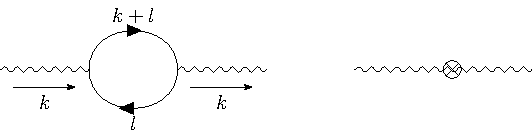
\includegraphics{Images/photoprop.pdf}
    \caption*{}
    \labfig{photoprop}
\end{figure}
\begin{align*}
i\pi^{\mu\nu}(k)=&(-1)(ig)^2\left(\frac{1}{i}\right)^2\int\frac{d^4l}{(2\pi)^4}\frac{\Tr{P_L(\slashed{l}+\slashed{k})\gamma^\mu P_LP_L\slashed{l}\gamma^\nu P_L}}{(l+k)^2l^2}\\
&-i(Z_3-1)(k^2g^{\mu\nu}-k^\mu k^\nu)+\pazocal{O}(g^4)
\end{align*}
Inside the trace in the numerator, we have $P_L^2=P_L$, $P_L\gamma^\mu=P_R\gamma^\mu$ and $P_L\gamma^\mu\gamma^\nu=\gamma^\mu\gamma^\nu P_L$ so all the $P_L$ can be collapsed into one, giving us:
\[
\Tr{P_L(\slashed{l}+\slashed{k})\gamma^\mu P_LP_L\slashed{l}\gamma^\nu P_L}=\Tr{(\slashed{l}+\slashed{k})\gamma^\mu\slashed{l}\gamma^\nu P_L}
\]
$P_L=(1-\gamma_5)/2$, the term with $1/2$ simply gives us half the result that we get with a Dirac field, the term with $-\gamma_5/2$ yields a vanishing contribution to $\pi^{\mu\nu}$:\marginnote{$\Tr{\gamma_5\gamma^\mu\gamma^\nu\gamma^\rho\gamma^\sigma}=-4i\epsilon^{\mu\nu\rho\sigma}$}
\[
-\frac{1}{2}\Tr{(\slashed{l}+\slashed{k})\gamma^\mu\slashed{l}\gamma^\nu\gamma_5}=2i\epsilon^{\alpha\mu\beta\nu}(l+k)_\alpha l_\beta=2i\epsilon^{\alpha\mu\beta\nu}k_\alpha l_\beta
\]
Therefore, what we have is:
\begin{align*}
\pi^{\mu\nu}(k)=&\frac{1}{2}\pi^{\mu\nu}(k)_{\text{Dirac}}-2g^2\epsilon^{\alpha\mu\beta\nu}k_\alpha\int\frac{d^4l}{(2\pi)^4}\frac{l_\beta}{(l+k)^2l^2}\\
&-(Z_3-1)(k^2g^{\mu\nu}-k^\mu k^\nu)+\pazocal{O}(g^4)
\end{align*}
The integral is logarithmically divergent, carries a single index $\beta$ and depends only on the vector $k$: it must be some quantity proportional to $k_\beta$. This contribution vanishes when contracted with $\epsilon^{\alpha\mu\beta\nu}k_\alpha$. At 1-loop level, the contribution to the photon propagator of a single charged Weyl field is half of that of a Dirac field,\marginnote{This is physically reasonable since a Dirac field is equivalent to two charged Weyl fields.} nothing interesting happens at this level.

We now bring our attention to diagrams with three external photons and no external fermions:
\begin{figure}[h]
    \centering
    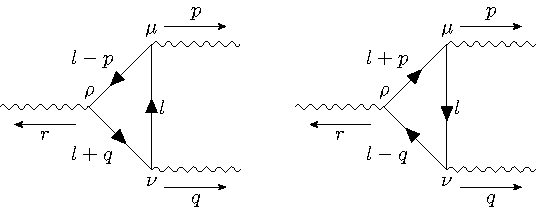
\includegraphics{Images/3photons.pdf}
    \caption*{}
    \labfig{3photons}
\end{figure}
\begin{align*}
iV^{\mu\nu\rho}(p,q,r)=&-\left(\frac{ig}{i}\right)^3\int\frac{d^4l}{(2\pi)^4}\frac{\Tr{(-\slashed{l}+\slashed{p})\gamma^\mu(-\slashed{l})\gamma^\nu(-\slashed{l}-\slashed{q})\gamma^\rho P_L}}{(l-p)^2l^2(l+q)^2}\\
&+(p,\mu\xleftrightarrow[]{}q,\nu)+\pazocal{O}(g^5)
\end{align*}
As before, the term in the numerator with $P_L\to1/2$ gives half the result that we get with a Dirac field, which makes a vanishing contribution to $V^{\mu\nu\rho}(p,q,r)$. We make the replacement $P_L\to-\gamma_5/2$ and we obtain:
\[
\Tr{(-\slashed{l}+\slashed{p})\gamma^\mu(-\slashed{l})\gamma^\nu(-\slashed{l}-\slashed{q})\gamma^\rho P_L}\to\Tr{(\slashed{l}-\slashed{p})\gamma^\mu\slashed{l}\gamma^\nu(\slashed{l}+\slashed{q})\gamma^\rho\frac{\gamma_5}{2}}
\]
We would like to have $V^{\mu\nu\rho}(p,q,r)$ gauge invariant, which means having:
\begin{equation}
\labeq{pqr}
\left\{
\begin{aligned}
&p_\mu V^{\mu\nu\rho}(p,q,r)=0 \\
&q_\nu V^{\mu\nu\rho}(p,q,r)=0 \\
&r_\rho V^{\mu\nu\rho}(p,q,r)=0
\end{aligned}
\right.
\end{equation}
We start by checking the last relation:
\begin{align*}
r_\rho N^{\mu\nu\rho}&=r_\rho\frac{1}{2}\Tr{(\slashed{l}-\slashed{p})\gamma^\mu\slashed{l}\gamma^\nu(\slashed{l}+\slashed{q})\gamma^\rho\gamma_5}\\
&=\frac{1}{2}\Tr{(\slashed{l}-\slashed{p})\gamma^\mu\slashed{l}\gamma^\nu(\slashed{l}+\slashed{q})r_\rho\gamma^\rho\gamma_5}\marginnote{Cyclic property of the trace.}\\
&=\frac{1}{2}\Tr{\slashed{l}\gamma^\nu(\slashed{l}+\slashed{q})\slashed{r}(\slashed{l}-\slashed{p})\gamma^\mu\gamma_5}\marginnote{$r+p+q=0\xleftrightarrow[]{}r=-(p+q)$}\\
&=\frac{1}{2}\Tr{\slashed{l}\gamma^\nu(\slashed{l}+\slashed{q})[-(\slashed{l}+\slashed{q})+(\slashed{l}-\slashed{p})](\slashed{l}-\slashed{p})\gamma^\mu\gamma_5}
\end{align*}
Where we have written $\slashed{r}$ in that clever way in order to simplify the equation:
\[
(\slashed{l}+\slashed{q})[-(\slashed{l}+\slashed{q})+(\slashed{l}-\slashed{p})](\slashed{l}-\slashed{p})=(l+q)^2(\slashed{l}-\slashed{p})-(l-p)^2(\slashed{l}+\slashed{q})
\]
Now we have:
\begin{align*}
r_\rho N^{\mu\nu\rho}=&\frac{1}{2}(l+q)^2\Tr{\slashed{l}\gamma^\nu(\slashed{l}-\slashed{p})\gamma^\mu\gamma_5}\\
&-\frac{1}{2}(l-p)^2\Tr{\slashed{l}\gamma^\nu(\slashed{l}+\slashed{q})\gamma^\mu\gamma_5}\\
=&-2i\epsilon^{\alpha\nu\beta\mu}[(l+q)^2l_\alpha(l-p)_\beta-(l-p)^2l_\alpha(l+q)_\beta]\\
=&2i\epsilon^{\alpha\nu\beta\mu}[(l+q)^2l_\alpha p_\beta+(l-p)^2l_\alpha q_\beta]
\end{align*}
With this result, we obtain:
\begin{align*}
r_\rho V^{\mu\nu\rho}(p,q,r)=&-2g^3\epsilon^{\alpha\nu\beta\mu}\int\frac{d^4l}{(2\pi)^4}\left[\frac{l_\alpha p_\beta}{l^2(l-p)^2}-\frac{l_\alpha q_\beta}{l^2(l+q)^2}\right]\\
&+(p,\mu\xleftrightarrow[]{}q,\nu)+\pazocal{O}(g^5)
\end{align*}
The first term in the integrand gives us a term proportional to $p_\alpha p_\beta$, the second one a term proportional to $q_\alpha q_\beta$: both of them vanish when contracted with $\epsilon^{\alpha\nu\beta\mu}$, hence $r_\rho V^{\mu\nu\rho}(p,q,r)=0$.\\
$iV^{\mu\nu\rho}(p,q,r)$ is not manifestly symmetric on the exchanges $(p,\mu\xleftrightarrow[]{}r,\rho)$ and $(q,\nu\xleftrightarrow[]{}r,\rho)$, so we have to compute the other two terms in \refeq{pqr}.

We repeat the same procedure for $p_\mu V^{\mu\nu\rho}(p,q,r)$ and what we find is:
\begin{align*}
p_\mu V^{\mu\nu\rho}(p,q,r)=&2g^3\epsilon^{\alpha\nu\beta\rho}\int\frac{d^4l}{(2\pi)^4}\left[\frac{l_\alpha q_\beta}{l^2(l+q)^2}-\frac{(l-p)_\alpha(p+q)_\beta}{(l-p)^2(l+q)^2}\right]\\
&+(p,\mu\xleftrightarrow[]{}q,\nu)+\pazocal{O}(g^5)
\end{align*}
The first term in the integrand gives us a term proportional to $q_\alpha q_\beta$, so it vanishes when contracted with $\epsilon^{\alpha\nu\beta\mu}$. For the second term, it is possible to make a shift $l\to l+p$:
\[
\frac{(l-p)_\alpha(p+q)_\beta}{(l-p)^2(l+q)^2}\to\frac{l_\alpha(p+q)_\beta}{l^2(l+p+q)^2}
\]
At this point, we can use the same argument as before, with the integral that must yields a term proportional to $(p+q)_\alpha(p+q)_\beta$ which vanishes when contracted with $\epsilon^{\alpha\nu\beta\mu}$, providing $p_\mu V^{\mu\nu\rho}(p,q,r)=0$. However, the integral is linearly divergent so things are not as easy as they seem. Let's make a simpler example to better understand this concept: consider a one-dimensional linearly divergent integral $I(a)$.
\[
I(a)=\int_{-\infty}^{+\infty}dxf(x+a)
\]
with $f(\pm\infty)=c_\pm$ ($c_+\neq c_-)$. If the integral had been convergent, $I(a)$ would not depend on $a$. In this case, we perform a Taylor expansion, obtaining:
\[
I(a)=\int_{-\infty}^{+\infty}dx\left[f(x)+af'(x)+\frac{1}{2}a^2f''(x)+\cdots\right]
\]
When integrating the derivatives at orders higher than one, they vanish since $f(\pm\infty)$ is a constant, so we are left with:
\[
I(a)=I(0)+a(c_+-c_-)
\]
We go back to our case:
\[
f_\alpha(l):=\frac{l_\alpha}{l^2(l+p+q)^2} \quad \int\frac{d^4l}{(2\pi)^4}f_\alpha(l)=A(p+q)
_\alpha
\]
Consider now $l\to l-p$:
\[
f_\alpha(l-p)=f_\alpha(l)-p^\beta\frac{\partial f_\alpha(l)}{\partial l^\beta}
\]
We know the contribution coming from the first term, so we bring our attention to the second term:
\begin{align*}
-p^\beta\int\frac{d^4l}{(2\pi)^4}\frac{\partial f_\alpha(l)}{\partial l^\beta}&\underset{\mathclap{\tikz \node {$\uparrow$} node [below=1ex] {\footnotesize  Wick's rotation};}}{=}-ip^\beta\lim_{l\to+\infty}\int\frac{dS_\beta}{(2\pi)^4}f_\alpha(l)\\
&=-ip^\beta\lim_{l\to+\infty}\int\frac{d\Omega}{(2\pi)^4}\frac{l^2l_\beta l_\alpha}{l^2(l+p+q)^2}\\
&=-ip^\beta\frac{\Omega_4}{(2\pi)^4}\frac{1}{4}g_{\alpha\beta}=-ip^\beta\frac{g_{\alpha\beta}}{32\pi^2}
\end{align*}
Combining all of this together, the final result is:
\[
\int\frac{d^4l}{(2\pi)^4}f_\alpha(l-p)=\int\frac{d^4l}{(2\pi)^4}\frac{(l-p)_\alpha}{(l-p)^2(l+q)^2}=A(p+q)_\alpha-\frac{i}{32\pi^2}p_\alpha
\]
At this point, we are ready to compute $p_\mu V^{\mu\nu\rho}(p,q,r)$:
\begin{align*}
p_\mu V^{\mu\nu\rho}(p,q,r)&=\frac{ig^3}{16\pi^2}\epsilon^{\alpha\nu\beta\rho}p_\alpha(p+q)_\beta+(p,\mu\xleftrightarrow[]{}q,\nu)+\pazocal{O}(g^5)\\
&=\frac{ig^3}{8\pi^2}\epsilon^{\alpha\nu\beta\rho}p_\alpha q_\beta+\pazocal{O}(g^5)
\end{align*}
Following analogous calculations, one also finds:
\[
q_\nu V^{\mu\nu\rho}(p,q,r)=\frac{ig^3}{8\pi^2}\epsilon^{\alpha\rho\beta\mu}q_\alpha p_\beta+\pazocal{O}(g^5)
\]
This shows that the three-photon vertex does not exhibit the expected symmetry among the external lines.\marginnote{\textit{"This concept is not easy to digest, it's not like arrosticini"}. Also, do not have arrosticini with vino rosso otherwise it is game over.} The gauge symmetry is not conserved, due to the fact that the integral we computed is divergent and making a shift changes its value. We can set $a_\mu=c(p_\mu-q_\mu)$ and write:
\begin{equation}
\labeq{pqr2}
\left\{
\begin{aligned}
&p_\mu V^{\mu\nu\rho}(p,q,r)=-\frac{ig^3}{8\pi^2}(1-c)\epsilon^{\nu\rho\alpha\beta}q_\alpha r_\beta+\pazocal{O}(g^5)\\
&q_\nu V^{\mu\nu\rho}(p,q,r)=-\frac{ig^3}{8\pi^2}(1-c)\epsilon^{\rho\mu\alpha\beta}r_\alpha p_\beta+\pazocal{O}(g^5)\\
&r_\rho V^{\mu\nu\rho}(p,q,r)=-\frac{ig^3}{8\pi^2}2c\epsilon^{\mu\nu\alpha\beta}p_\alpha q_\beta+\pazocal{O}(g^5)
\end{aligned}
\right.
\end{equation}
It is easy to see that it is not possible to choose a value of $c$ that cancels all the anomalies: we have failed in constructing a gauge-invariant U(1) theory with a single charged Weyl field.

Consider now a U(1) gauge theory with multiple left-handed charged Weyl fields $\psi_i$ with charges $Q_i$, the covariant derivative is $(\partial_\mu-igQ_iA_\mu)\psi_i$. Each vertex gains an extra factor $Q_i$, so the right-hand sides of \refeq{pqr2} gets multiplied by a factor $\sum_i Q_i^3$: if this sum happens to be zero, then gauge invariance is restored. The simplest possible case is to have the fields coming in pairs with equal and opposite charges, but we can also have one field with charge +2 and eight fields with charge -1.
We can generalize this idea to non-abelian gauge theories. Suppose to have a single Weyl field in a representation R: we gain an extra factor $\Tr{T_R^aT_R^bT_R^c}$\marginnote{Indices $a,b,c$ go along with $p,q,r$.}. Combining it with $P_L$ gives us:
\begin{center}
\begin{tikzcd}
&\frac{1}{2}\Tr{[T_R^a,T_R^b]T_R^c}=\frac{i}{2}T(R)f^{abc}T_R^c\\
P_L=\frac{1-\gamma_5}{2} \arrow[ru, "1/2"] \arrow[rd, "-\gamma_5/2"] \\
& \frac{1}{2}\Tr{T_R^a\{T_R^b,T_R^c\}}=A(\text{R})d^{abc}
\end{tikzcd}
\end{center}
The $1/2$ term contributes to the renormalization of the tree-level three-gluon vertex, for the $\gamma_5$ term we have the completely symmetric tensor $d^{abc}$ and $A(\text{R})$ which is the anomaly coefficient of the representation R. In order for this theory to exist, it must be $A(\text{R})=0$: a theory with left-handed Weyl fields coming in R$\oplus\overline{\text{R}}$ is automatically anomaly free since $A(\overline{\text{R}})=-A$(R). In all the other cases, we must arrange the cancellation by hand. For SU(2) and SO(N), all representations have $A($R)=0, for SU(N) with N>3 the cancellation is not trivial.

We have to check that the SM is anomaly free. The gauge group is G=SU$(3)_{\text{C}}\times$SU$(2)_{\text{L}}\times$U$(1)_{\text{Y}}$.
\[
\left\{
\begin{aligned}
&\text{U}(1)_{\text{Y}}^3=\sum_i[(2Y_{L_i}^3-Y_{e_i}^3)+3(2Y_{Q_i}^3-Y_{u_i}^3-Y_{d_i}^3)]=0\\
&\text{SU}(2)_{\text{L}}^3=0 \qquad \text{SU}(3)_{\text{C}}^3=0\\
&\text{SU}(3)_{\text{C}}\text{SU}(2)_{\text{L}}\text{U}(1)_{\text{Y}}=\Tr{T_{\text{SU}(3)_{\text{C}}}[T_{\text{SU}(2)_{\text{L}}},T_{\text{U}(1)_{\text{Y}}}]}\propto\Tr{T_{\text{SU}(3)_{\text{C}}}}=0\\
&\text{SU}(3)_{\text{C}}\text{U}(1)_{\text{Y}}^2, \text{SU}(2)_{\text{L}}\text{U}(1)_{\text{Y}}^2, \text{SU}(3)_{\text{C}}\text{SU}(2)_{\text{L}}^2, \text{SU}(3)_{\text{C}}^2\text{SU}(2)_{\text{L}}=0\\
&\text{SU}(3)_{\text{C}}^2\text{U}(1)_{\text{Y}}=\sum_i(-6Y_{Q_i}-3Y_{u_i}-3Y_{d_i})=0\\
&\text{SU}(2)_{\text{L}}^2\text{U}(1)_{\text{Y}}=\sum_i(2Y_{L_i}+6Y_{Q_i})=0
\end{aligned}
\right.
\]
\subsection{Anomalies in Global Symmetries}\marginnote{From \cite{Sr}, Chapter 76.}
The simplest example is QED with a massless Dirac field $\Psi$ with charge $Q=+1$ and Lagrangian given by:
\[
\pazocal{L}=-\frac{1}{4}F^{\mu\nu,a}F_{\mu\nu}^a+i\overline{\Psi}(\slashed{\partial}-igA)\Psi\marginnote{We call the coupling constant $g$ instead of $e$ because we are using this theory as a formal example rather than a physical one.}
\]
This Lagrangian is invariant under a U(1) transformation:
\[
\left\{
\begin{aligned}
&\Psi\to e^{-i\alpha(x)}\Psi\\
&\overline{\Psi}\to e^{+i\alpha(x)}\overline{\Psi}\\
&A_\mu(x)\to A_\mu(x)+\partial_\mu\alpha(x)
\end{aligned}
\right.
\]
From which we obtain the conserved current $J^\mu=\overline{\Psi}\gamma^\mu\Psi$. Due to the absence of the mass term, we also have an axial symmetry U$(1)_{\text{A}}$:
\[
\left\{
\begin{aligned}
&\Psi\to e^{-i\beta\gamma_5}\Psi\\
&\overline{\Psi}\to e^{+i\beta\gamma_5}\overline{\Psi}
\end{aligned}
\right.
\]
This result in a current $J_A^\mu=\overline{\Psi}\gamma^\mu\gamma_5\Psi$ which is not conserved but instead has a divergence:
\begin{equation}
\labeq{curr}
\partial_\mu J^\mu_A=-\frac{g^2}{16\pi^2}\epsilon^{\mu\nu\rho\sigma}F_{\mu\nu}F_{\rho\sigma}
\end{equation}
To prove this, consider the matrix element $\bra{p,q}J_A^\rho(x)\ket{0}$ where $\bra{p,q}$ is a state of two outgoing photons with four-momenta $p,q$ and polarizations $\varepsilon_\mu,\varepsilon_\nu'$. The LSZ formula for photons tells us that we can express this matrix element as:
\begin{equation}
\labeq{me}
(ig)^2\varepsilon_\mu\varepsilon_\nu'\int d^4xd^4ye^{-i(px+qy)}\bra{0}T[J^\mu(x)J^\nu(y)J^\rho_A(z)]\ket{0}
\end{equation}
$J^\mu(x)$ and $J^\nu(y)$ are the usual N\"other currents corresponding to the U(1) gauge symmetry. We then expect to recover Ward identities:
\[
\left\{
\begin{aligned}
&\frac{\partial}{\partial x^\mu}\bra{0}T[J^\mu(x)J^\nu(y)J^\rho_A(z)]\ket{0}=0\\
&\frac{\partial}{\partial y^\nu}\bra{0}T[J^\mu(x)J^\nu(y)J^\rho_A(z)]\ket{0}=0\\
&\frac{\partial}{\partial z^\rho}\bra{0}T[J^\mu(x)J^\nu(y)J^\rho_A(z)]\ket{0}=0
\end{aligned}
\right.
\]
Using the last equation in \refeq{me} we should have:
\[
\frac{\partial}{\partial z^\rho}\bra{p,q}J_A^\rho(x)\ket{0}=0
\]
However, what we learnt so far has taught us to proceed more cautiously. Define now $C^{\mu\nu\rho}(p,q,r)$ via:
\[
(2\pi)^4\delta(p+q+r)C^{\mu\nu\rho}(p,q,r)=\int d^4xd^4yd^4ze^{-i(px+qy+rz)}\bra{0}T[J^\mu(x)J^\nu(y)J^\rho_A(z)]\ket{0}
\]
We can rewrite \refeq{me} as:
\[
\bra{p,q}J_A^\rho(x)\ket{0}=-g^2\varepsilon_\mu\varepsilon_\nu'C^{\mu\nu\rho}(p,q,r)e^{irz}\Bigr|_{\substack{r=-p-q}}
\]
By taking the divergence of the current, the Ward identities become:
\[
\left\{
\begin{aligned}
&p_\mu C^{\mu\nu\rho}(p,q,r)=0\\
&q_\nu C^{\mu\nu\rho}(p,q,r)=0\\
&r_\rho C^{\mu\nu\rho}(p,q,r)=0
\end{aligned}
\right.
\]
The vertex function $iV^{\mu\nu\rho}(p,q,r)$ previously computed is related to $C^{\mu\nu\rho}(p,q,r)$ by:
\[
iV^{\mu\nu\rho}(p,q,r)=-\frac{1}{2}(ig)^3C^{\mu\nu\rho}(p,q,r)+\pazocal{O}(g^5)
\]
We definitely want to preserve the first two Ward identities because they imply conservation of currents coupled to gauge fields, which is necessary for gauge invariance. Preserving these two results in:
\[
r_\rho C^{\mu\nu\rho}(p,q,r)=-\frac{i}{2\pi^2}\epsilon^{\mu\nu\alpha\beta}p_\alpha q_\beta+\pazocal{O}(g^2)
\]
Using this result we finally get:
\[
\bra{p,q}J_A^\rho(x)\ket{0}=-\frac{g^2}{2\pi^2}\epsilon^{\mu\nu\alpha\beta}p_\alpha q_\beta\varepsilon_\mu\varepsilon_\nu'e^{-i(p+q)z}+\pazocal{O}(g^4)
\]
The right-hand side of this equation is exactly what we get in the free-field theory for the matrix element of the right-hand side of \refeq{curr}, which is correct up to possible higher order corrections.
\section{Effective Field Theory (EFT) for Goldstone Bosons}
\labsec{eft}
\marginnote{From \cite{P}, Section 2.4 and Section 4.2.\\
From \cite{SS}, Sections 3.3, 3.4, 3.6 and 3.7.}
The Goldstone nature of the pseudoscalar mesons implies strong constraints on their interactions. Since there is a mass gap separating the pseudoscalar octet from the rest of the spectrum, it is possible to build an EFT containing only the Goldstone bosons.\\
An EFT is characterized by some effective Lagrangian:
\[
\pazocal{L}_{\text{EFT}}=\pazocal{L}^{(4)}+\sum_n C^{(n)}O^{(n)}(x)
\]
where $O^{(n)}(x)$ are operators constructed with the light fields and the information on any heavy degrees of freedom is hidden in the coefficients $C^{(n)}$. The
operators $O^{(n)}$ are usually organized according to their dimension $d_n$, which fixes the dimension of their coefficients.
\[
[O^{(n)}]=d_n\to C^{(n)}\sim\frac{1}{\Lambda^{d_n-4}}
\]
with $\Lambda$ some characteristic heavy state of the system. At energies below $\Lambda$, the behaviour of different operators is determined by their dimension. It is possible to distinguish three type of operators:
\begin{itemize}
    \item Relevant, $d_n<4$
    \item Marginal, $d_n=4$
    \item Irrelevant, $d_n>4$
\end{itemize}
They are irrelevant because their effects are suppressed by powers of $E/\Lambda$ and are therefore small at low energies.\marginnote{This does not mean that they are not important, they usually contain the interesting information about the underlying dynamics at higher
scales. The point is that irrelevant operators are weak at low energies.}\\
In an EFT, we have to specify the degrees of freedom, the symmetry group, the range of validity and then write the most general Lagrangian. There are three possible different outcomes:
\begin{enumerate}
    \item The UV theory is unknown, e.g. the Standard Model
    \item The UV theory is known and it is possible to perform \textit{matching}
    \item The UV theory is known but performing \textit{matching} is not possible
\end{enumerate}
We now want to study the following case:
\[
\text{G}=\text{SU}(3)_{\text{L}}\times\text{SU}(3)_{\text{R}}\to\text{H=SU}(3)_{\text{V}}
\]
Geometrically, the Goldstone bosons are the coordinates of the coset G/H denoted by $\phi^a(a=1,\cdots,8)$ 
% Consider two elements, $g\in\text{G}$ and $h\in\text{H}$. Any $g\in\text{G}$ can be decomposed as $g=\xi\cdot h$ with $\xi\in\text{G}$. What we are interested in are transformation properties of $\xi(\phi)$:
% \[
% g\xi(\phi)=g'=\xi(\phi')h(g,\phi)\Rightarrow\xi(\phi)\to\xi(\phi')=g\xi(\phi)h^{-1}(g,\phi)
% \]
and we choose a coset representative $\overline{\xi}(\phi)=(\xi_L(\phi),\xi_R(\phi))\in\text{G}$. The change of the Goldstone coordinates under a chiral transformation $g=(g_L,g_R)\in\text{G}$ is given by:
\[
\xi_L(\phi)\to g_L\xi_L(\phi)h^\dagger(\phi,g) \quad \xi_R(\phi)\to g_R\xi_R(\phi)h^\dagger(\phi,g)
\]
where $h(\phi,g)\in\text{H}$. Since the same transformation $h(\phi,g)$ occurs both in the left and in the right sector we can get rid of it by combining the two chiral relations in a simpler form:
\[
U(\phi):=\xi_R(\phi)\xi_L^\dagger(\phi) \quad U(\phi)\to g_RU(\phi)g_L^\dagger
\]
Without loss of generality, we can take a canonical choice of coset representative such that $\xi_L^\dagger(\phi)=\xi_R(\phi):=u(\phi)$. The $3\times3$ unitary matrix $U(\phi)$ becomes:
\[
U(\phi)=u^2(\phi)=\exp{i\sqrt{2}\frac{\Phi}{f}}
\]
This gives a very convenient parametrization of the Goldstone fields:
\[
\Phi(x):=\sum_{a=1}^8\frac{\lambda^a}{\sqrt{2}}\phi^a=\frac{1}{\sqrt{2}}\left(\begin{array}{ccc}
    \phi_3+\phi_8/\sqrt{3} & \phi_1-i\phi_2 & \phi_4-i\phi_5 \\
    \phi_1+i\phi_2 & -\phi_3-\phi_8/\sqrt{3} & \phi_6-i\phi_7 \\
    \phi_4+i\phi_5 & \phi_6+i\phi_7 & -2\phi_8/\sqrt{3} \\
\end{array}\right)
\]
We now want to look at the commutator of this object with the charge, which at low energy is given by:
\[
Q=\mqty(\dmat{+2/3,-1/3,-1/3})\to[Q,\Phi]=\left(\begin{array}{ccc}
    0 & +\Phi_{12} & +\Phi_{13} \\
    -\Phi_{21} & 0 & 0 \\
    -\Phi_{31} & 0 & 0
\end{array}\right)
\]
The entries with zero correspond to Goldstone bosons with zero charge while the non-zero entries are charged Goldstone bosons. To correctly associate entries with Goldstone bosons we can use the strangeness generator:
\[
S=\mqty(\dmat{0,0,1})\to[S,\Phi]=\left(\begin{array}{ccc}
    0 & 0 & -\Phi_{13} \\
    0 & 0 & -\Phi_{23} \\
    +\Phi_{31} & +\Phi_{32} & 0
\end{array}\right)
\]
It then follows that:
\begin{equation}
\labeq{Phi}
\Phi(x):=\frac{\lambda^a}{\sqrt{2}}\phi^a=\left(\begin{array}{ccc}
    \frac{\pi^0}{\sqrt{2}}+\frac{\eta_8}{\sqrt{6}} & \pi^+ & K^+ \\
    \pi^- & -\frac{\pi^0}{\sqrt{2}}+\frac{\eta_8}{\sqrt{6}} & K^0 \\
    K^- & \overline{K}^0 & -2\frac{\eta_8}{\sqrt{6}}
\end{array}\right)
\end{equation}
To get a low energy Lagrangian of QCD for the light quark sector $(u, d, s)$, we should write the most general Lagrangian involving the matrix $U(\phi)$ which is consistent with chiral symmetry. Due to the unitarity of the $U$ matrix, at least two derivative are required in order to generate a non-trivial interaction. To lowest order, this is given by:
\[
\pazocal{L}=\frac{f^2}{4}\Tr{\partial_\mu U\partial^\mu U^\dagger}
\]
The factor $1/4$ is for normalization, the parameter $f^2$ is needed to get dimension 4 and it will later be related to the pion decay $\pi^+\to\mu^+\nu_\mu$.\\
The multiplicative constant $f^2/4$ generates the standard form of the kinetic term, which can be seen by expanding $U(\phi)$ in power series of $\Phi$:
\[
U\simeq1+i\sqrt{2}\frac{\Phi}{f}+\cdots \qquad \partial_\mu U\simeq i\sqrt{2}\partial_\mu\frac{\Phi}{f}
\]
This results in:
\[
\begin{aligned}
\pazocal{L}&=\frac{f^2}{4}\Tr{-i\sqrt{2}\partial_\mu\frac{\Phi}{f}i\sqrt{2}\partial^\mu\frac{\Phi}{f}}+\cdots=\frac{1}{4}\Tr{\lambda^a\partial_\mu\phi^a\lambda^b\partial^\mu\phi^b}+\cdots\\
&=\frac{1}{4}\partial_\mu\phi^a\partial^\mu\phi^b\underbrace{\Tr{\lambda_a\lambda_b}}_{=2\delta^{ab}}+\cdots=\frac{1}{2}\partial_\mu\phi^a\partial^\mu\phi^a+\cdots
\end{aligned}
\]
Our Lagrangian is invariant under a global SU$(3)_{\text{L}}\times$SU$(3)_{\text{R}}$ transformation:
\begin{equation}
\labeq{t1}
U\to RUL^\dagger \qquad U^\dagger\to LU^\dagger R^\dagger
\end{equation}
and we now want to see the vector and axial currents associated with this symmetry just like we did in \refsec{symmqcd}. To this purpose, we parametrize $L$ and $R$ as:
\[
L=\exp{-i\theta_a^L\frac{\lambda^a}{2}} \qquad R=\exp{-i\theta_a^R\frac{\lambda^a}{2}} 
\]
To get $J_L^{\mu,a}$, set $\theta_a^R=0$. At first order in $\theta_a^L$ we get:
\[
\left\{
\begin{aligned}
&U\to RUL^\dagger=U\left(1+i\theta_a^L\frac{\lambda_a}{2}\right) &&U^\dagger\to LU^\dagger R^\dagger=\left(1-i\theta_a^L\frac{\lambda_a}{2}\right)U^\dagger\\
&\partial_\mu U\to\partial_\mu U\left(1+i\theta_a^L\frac{\lambda_a}{2}\right)+Ui\partial_\mu\theta_a^L\frac{\lambda_a}{2} && \partial^\mu U^\dagger\to\left(1-i\theta_a^L\frac{\lambda_a}{2}\right)\partial^\mu U^\dagger-i\partial^\mu\theta^L_a\frac{\lambda_a}{2}U^\dagger
\end{aligned}
\right.
\]
From this, we obtain:
\[
\begin{aligned}
\delta\pazocal{L}&=\frac{f^2}{4}\Tr{Ui\partial_\mu\theta_a^L\frac{\lambda_a}{2}\partial^\mu U^\dagger-\partial_\mu Ui\partial^\mu\theta_a^L\frac{\lambda_a}{2}U^\dagger}\\
&=\frac{f^2}{4}i\partial_\mu\theta_a^L\Tr{\frac{\lambda_a}{2}[U(\partial^\mu U^\dagger)-(\partial^\mu U)U^\dagger]}\\
&=\frac{f^2}{4}i\partial_\mu\theta_a^L\Tr{\lambda_a(\partial^\mu U^\dagger)U}
\marginnote{In the last step, we used:
\[
\partial_\mu(UU^\dagger)=0=(\partial_\mu U)U^\dagger+U(\partial_\mu U^\dagger)
\]
from which it follows:
\[
U(\partial_\mu U^\dagger)=-(\partial_\mu U)U^\dagger
\]}
\end{aligned}
\]
Using \refeq{currents}, for the left currents we have:
\begin{equation}
\labeq{jl}
J_L^{\mu,a}=\frac{\partial\delta\pazocal{L}}{\partial\partial_\mu\theta_a^L}=i\frac{f^2}{4}\Tr{\lambda_a(\partial^\mu U^\dagger)U}
\end{equation}
In the same way, by setting $\theta_a^L=0$, for the right currents one gets:
\begin{equation}
\labeq{jr}
J_R^{\mu,a}=\frac{\partial\delta\pazocal{L}}{\partial\partial_\mu\theta_a^R}=-i\frac{f^2}{4}\Tr{\lambda_aU(\partial^\mu U^\dagger)}
\end{equation}
Combining these two results gives us the vector and axial currents:
\[
\left\{
\begin{aligned}
&J_V^{\mu,a}=J_R^{\mu,a}+J_L^{\mu,a}=-i\frac{f^2}{4}\Tr{\lambda_a[U,\partial^\mu U^\dagger]}\\
&J_A^{\mu,a}=J_R^{\mu,a}-J_L^{\mu,a}=-i\frac{f^2}{4}\Tr{\lambda_a\{U,\partial^\mu U^\dagger\}}
\end{aligned}
\right.
\]
Because of the SU$(3)_{\text{L}}\times$SU$(3)_{\text{R}}$ symmetry, both currents are conserved. The vector currents contain terms with an even number of Goldstone bosons while the axial currents, on the other hand, are odd in the number of Goldstone bosons.\marginnote[-1cm]{To see that, send $\Phi\to-\Phi$ and notice how $J_V^{\mu,a}$ goes to $J_\V^{\mu,a}$ while $J_A^{\mu,a}$ goes to $-J_V^{\mu,a}$.}\\
% \[
% \pazocal{L}=\frac{1}{2}\Braket{\partial_\mu\Phi\partial^\mu\Phi}+\frac{1}{12f^2}\Braket{(\Phi\overset{\leftrightarrow}{\partial_\mu}\Phi)(\Phi\overset{\leftrightarrow}{\partial^\mu}\Phi)}+\pazocal{O}(\Phi^6/f^4)
% \]
So far, we assumed a perfect SU$(3)_{\text{L}}\times$SU$(3)_{\text{R}}$ symmetry but we have seen in \refsec{symmqcd} that the quark mass term results in explicit symmetry breaking.
\[
M=\mqty(\dmat{m_u,m_d,m_s}) \qquad \pazocal{L}_{\text{M}}=-\overline{q}_RMq_L-\overline{q}_LMq_R
\]
$M$ is just a constant matrix and does not transform with the quark fields, but $\pazocal{L}_{\text{M}}$ would be invariant if $M$ transformed as:
\begin{equation}
\labeq{t2}
M\to RML^\dagger
\end{equation}
The most general Lagrangian invariant under \refeq{t1} and \refeq{t2} is given, at lowest order in $M$, by:
\[
\pazocal{L}_{\text{s.b.}}=\frac{f^2B_0}{2}\Tr{MU^\dagger+UM^\dagger}
\]
$B_0$ is a constant which, like $f$, is not fixed by symmetry requirements alone and cannot be predicted form the UV theory. Moreover, being $M=M^\dagger$, $\pazocal{L}_{\text{s.b.}}$ contains only terms even in the number of fields.\\
In order to determine the masses of the Goldstone bosons, one expands the Lagrangian above in powers of $\Phi$ and look at the terms of second order in the fields:
\[
\pazocal{L}=\frac{f^2B_0}{2}\Tr{M(U+U^\dagger)}=B_0\left\{-\Tr{M\Phi^2}+\pazocal{O}(\Phi^4/f^2)\right\}
\]
Using \refeq{Phi}, after some slightly annoying calculations the trace term reads:
\[
\begin{aligned}
\Tr{M\Phi^2}=&\pi^+\pi^-(m_u+m_d)+K^+K^-(m_u+m_s)+K^0\overline{K}^0(m_d+m_s)\\
&+\pi^0\pi^0(m_u+m_d)+\frac{1}{3}\eta_8^2(m_u+m_d+4m_s)+\frac{2}{\sqrt{3}}\pi^0\eta_8(m_u-m_d)
\end{aligned}
\]
To lowest order, the masses of the Goldstone bosons are given by:
\[
\marginnote{In the isospin-symmetric limit, $m_u=m_d$, so that there is no $\pi^0-\eta_8$ mixing and the parameter $\varepsilon$ vanishes.}
\left\{
\begin{aligned}
&m_{\pi^\pm}^2=(m_u+m_d)B_0 &&m_{\pi^0}^2=(m_u+m_d)B_0-\varepsilon+\pazocal{O}(\varepsilon^2)\\
&m_{K^\pm}^2=(m_u+m_s)B_0 &&m_{\eta^8}^2=\frac{1}{3}(m_u+m_d+4m_s)B_0+\varepsilon+\pazocal{O}(\varepsilon^2)\\
&m_{K^0}^2=(m_d+m_s)B_0 &&\varepsilon=\frac{B_0}{2}\frac{(m_u-m_d)^2}{2m_s-m_u-m_d}
\end{aligned}
\right.
\]
Although chiral symmetry alone cannot fix the absolute values of the
quark masses, it gives information about quark–mass ratios. Neglecting
the tiny $\pazocal{O}(\varepsilon)$ effects, one gets:
\[
\left\{
\begin{aligned}
&\frac{(m_{K^0}^2-m_{K^+}^2)-(m_{\pi^0}^2-m_{\pi^\pm}^2)}{m_{\pi^0}^2}=\frac{m_d-m_u}{m_d+m_u}=0.29\\
&\frac{m_{K^0}^2-m_{\pi^0}^2}{m_{\pi^0}^2}=\frac{2m_s-m_u-m_d}{2(m_u+m_d)}=12.6
\end{aligned}
\right.
\]
These two formulas imply the quark-mass ratios advocated by Weinberg:
\[
m_u:m_d:m_s=0.55:1:20.3
\]
Quark-mass corrections are therefore dominated by $m_s$.
\subsection{Coupling to External Currents}\marginnote{From \cite{SS}, Section 1.5.}
We now introduce into the Lagrangian of QCD the couplings to the eight vector and axial currents as well as the scalar and pseudo-scalar quark densities:
\begin{equation}
\labeq{lqcd}
\pazocal{L}_{\text{QCD}}=\pazocal{L}_{\text{QCD}}^0+\overline{q}\gamma^\mu(v_\mu+\gamma_5a_\mu)q-\overline{q}(s-i\gamma_5p)q
\end{equation}
This is the most general possible Lagrangian including external currents, the ordinary QCD Lagrangian is recovered by setting $v_\mu=a_\mu=p=0$ and $s=\text{diag}(m_u,m_d,m_s)$. Moreover, these currents can be used to incorporate the electromagnetic and semileptonic weak interactions, and the explicit breaking of chiral symmetry through the quark masses. The coupling of quarks to an external electromagnetic field $A_\mu$ is given by:
\[
r_\mu=v_\mu+a_\mu=eQA_\mu \quad l_\mu=v_\mu-a_\mu=eQA_\mu \quad Q=\text{diag}(+2/3,-1/3,-1/3)
\]
In the description of semileptonic interactions such as pion or neutron decay, one needs the interaction of quarks with the massive charged weak bosons $W_\mu^\pm$:
\begin{equation}
\labeq{lmu}
r_\mu=0 \quad l_\mu=-\frac{g}{\sqrt{2}}(W_\mu^+T_++\text{h.c.}) \quad T_+=\left(\begin{array}{ccc}
    0 & V_{ud} & V_{us} \\
    0 & 0 & 0 \\
    0 & 0 & 0
\end{array}\right)
\end{equation}
By using projection operators, the Lagrangian in \refeq{lqcd} can be written as:
\[
\begin{aligned}
\pazocal{L}_{\text{QCD}}=&\pazocal{L}_{\text{QCD}}^0+\overline{q}_L\gamma^\mu l_\mu q_L+\overline{q}_R\gamma^\mu r_\mu q_R-\overline{q}_R(s+ip)q_L-\overline{q}_L(s-ip)q_R
\end{aligned}
\]
Inserting now the current $l_\mu$ relative to the interaction of quarks with massive charged weak bosons into the Lagrangian above one obtains the standard
charged-current weak interaction in the light quark sector:
\begin{equation}
\labeq{weakinteraction}
\pazocal{L}=-\frac{g}{2\sqrt{2}}\left\{W_\mu^+[V_{ud}\overline{u}\gamma^\mu(1-\gamma_5)d+V_{us}\overline{u}\gamma^\mu(1-\gamma_5)s]+\text{h.c.}\right\}
\end{equation}
In presence of such currents, we define the covariant derivative and the field strength tensors as follows:
\[
\left\{
\begin{aligned}
&D_\mu U=\partial_\mu U-ir_\mu U+iUl_\mu &&D_\mu U^\dagger=\partial_\mu U^\dagger+iU^\dagger r_\mu-il_\mu U^\dagger\\
&F_{\mu\nu}^L=\partial_\mu l_\nu-\partial_\nu l_\mu-i[l_\mu,l_\nu] &&F^{\mu\nu}_R=\partial_\mu r_\nu-\partial_\nu r_\mu-i[r_\mu,r_\nu]
\end{aligned}
\right.
\]
Lastly, we introduce the linear combination with the scalar and the pseudo-scalar external fields $\chi=2B_0(s+ip)$. The most
general, locally invariant, effective Lagrangian at lowest chiral order is finally given by:
\begin{equation}
\labeq{l2}    
\pazocal{L}=\frac{f^2}{4}\Tr{D_\mu UD^\mu U^\dagger}+\frac{f^2}{4}\Tr{\chi U^\dagger+U\chi^\dagger} 
\end{equation}
which contains two free parameters: the pion decay constant $f$ and $B_0$, hidden in $\chi$.
\subsection{Charged Pion Decay}
A phenomenological application of all this machinery is the charged pion decay $\pi^+\to\mu^+\nu_\mu$. This is described by the annihilation of a $u$ quark and a $\overline{d}$ anti-quark into a $W^+$ boson, propagation of the $W^+$ boson and creation of $\mu^+$ and $\nu_\mu$ in the final state.
\begin{figure}[h]
    \centering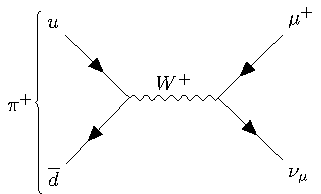
\includegraphics[width=0.45\textwidth]{Images/piondecay.pdf}
    \caption*{}
    \labfig{piondecay}
\end{figure}\\
Consider now the first term of \refeq{l2}, set $r_\mu=0$ with arbitrary $l_\mu$ which gets parametrized as:
\[
l_\mu=\sum_{a=1}^8\frac{\lambda_a}{2}l_\mu^a
\]
By explicitly computing the trace, the term linear in $l_\mu$ reads:
\[
\pazocal{L}_{\text{int}}=\sum_{a=1}^8l_\mu^ai\frac{f^2}{4}\Tr{\lambda_a(\partial^\mu U^\dagger)U}=\sum_{a=1}^8l_\mu^aJ_L^{\mu,a}
\]
where in the last step we used \refeq{jl} to define $J_L^{\mu,a}$. Expanding $U$ to first order $\Phi$ and using \refeq{Phi}, $J_L^{\mu,a}$ gets written as:
\[
\begin{aligned}
J_L^{\mu,a}&=i\frac{f^2}{4}\Tr{\lambda_a(\partial^\mu U^\dagger)U}\simeq i\frac{f^2}{4}\Tr{\lambda_a\left(-i\frac{\sqrt{2}}{f}\partial^\mu\Phi\right)}=\frac{f}{2}\partial^\mu\phi^a
\end{aligned}
\]
Inserting now the expression of $l_\mu$ from \refeq{lmu}, we get that the interaction term of a single Goldstone boson with a $W$ is the following:
\[
\pazocal{L}_{W\phi}=\Tr{l_\mu J^\mu_L}=-\frac{gf}{2\sqrt{2}}[W_\mu^+\Tr{T_+\partial^\mu\phi}+W_\mu^-\Tr{T_-\partial^\mu\phi}]
\]
Computing the trace term gives us:
\begin{align*}
\Tr{T_+\partial^\mu\phi}&=\left(\begin{array}{ccc}
    0 & V_{ud} & V_{us} \\
    0 & 0 & 0 \\
    0 & 0 & 0
\end{array}\right)\partial^\mu\left(\begin{array}{ccc}
    \frac{\pi^0}{\sqrt{2}}+\frac{\eta_8}{\sqrt{6}} & \pi^+ & K^+ \\
    \pi^- & -\frac{\pi^0}{\sqrt{2}}+\frac{\eta_8}{\sqrt{6}} & K^0 \\
    K^- & \overline{K}^0 & -2\frac{\eta_8}{\sqrt{6}} \\
\end{array}\right)\\
&=(V_{ud}\partial^\mu\pi^-+V_{us}\partial^\mu K^-)
\end{align*}
Putting everything together we end up with:
\[
\pazocal{L}_{W\phi}=-\frac{gf}{2\sqrt{2}}[W_\mu^+(V_{ud}\partial^\mu\pi^-+V_{us}\partial^\mu K^-)+W_\mu^-(V_{ud}^*\partial^\mu\pi^++V_{us}^*\partial^\mu K^+)]
\]
Neglecting higher order terms, the Feynman rule for the invariant amplitude of the pion decay reads:
\begin{align*}
\pazocal{M}&=\left(-i\frac{g}{\sqrt{2}}\overline{u}_{\nu_\mu}\gamma^\beta\frac{1-\gamma_5}{2}v_{\mu^+}\right)i\frac{g_{\beta\alpha}}{m_W^2}\left(-i\frac{gf}{2}V_{ud}^*(-ip^\alpha)\right)\\
&=-G_{\text{F}}V_{ud}f\overline{u}_{\nu_\mu}\slashed{p}(1-\gamma_5)v_{\mu^+}
\end{align*}
where $p$ denotes the pion four-momentum.
From this, it is possible to evaluate the decay rate by explicit calculations:
\begin{align*}
\Gamma=\frac{1}{\tau}&=\frac{1}{2m_{\pi^+}}\int\frac{d^3p_{\nu_\mu}}{2E_{\nu_\mu}}\frac{d^3p_{\mu^+}}{2E_{\mu^+}}\sum_{\text{pol}}|\pazocal{M}|^2(2\pi)^4\delta^4(p_{\pi^+}-p_{\nu_\mu}-p_{\mu^+})\\
&=\frac{G_{\text{F}^2}|V_{ud}|^2}{4\pi}f^2m_\mu^2m_\pi\left[1-\frac{m_\mu^2}{m_\pi^2}\right]^2
\end{align*}
The constant $f$ is referred to as the pion-decay constant in the chiral limit, it measures the strength of the matrix element of the axial current
operator between a one-Goldstone-boson state and the vacuum. From the measurement of the decay rate, one gets for the pion-decay constant the value of $f=92.4$\,MeV.
Once we know the decay, it is also possible to test the lepton flavour universality:
\[
R_{e\mu}:=\frac{\Gamma(\pi^+\to e^+\nu_e)}{\Gamma(\pi^+\to\mu^+\nu_\mu)}=\left(\frac{m_e}{m_\mu}\right)^2\left[\frac{1-m_e^2/m_\pi^2}{1-m_\mu^2/m_\pi^2}\right]=1.283\cdot10^{-4}
\]
\section{Semileptonic Decays of Light Hadrons}\marginnote{From \cite{GT}, Section 7.3 and Section 8.}
\subsection{Measuring $V_{ud}$}
Phenomenologically, the key process to measure the $d\to u$ transitions is the $\beta$-decay, which comes in three different forms:
\begin{itemize}
    \item nuclear $\beta$ decay, e.g. $^3$H$\to^3$He or $^{14}$C$\to^{14}$N
    \item neutron $\beta$ decay, $n\to pe^-\overline{\nu}_e$
    \item pion $\beta$ decay, $\pi^+\to\pi^0e^+\nu_e$ or $\pi^-\to\pi^0e^-\overline{\nu}_e$
\end{itemize}
We start our discussion by considering the \textbf{nuclear $\mathbf{\beta}$ decay} and it is possible to use symmetry arguments in order to make our life easier. The idea is to determine the matrix element of an operator $O_\beta$ sandwiched between two spin-0 states $N$ and $N'$.
\[
\bra{N}O_\beta\ket{N'}
\]
$O_\beta$ comes from $W$ exchange, so it can be vector or axial. The vector and axial currents are, respectively, even and odd under parity. The external states have a definite parity and, since QCD respects parity, only one of the vector or axial currents can be non-vanishing. This means fewer matrix elements to calculate which makes us happy. \raisebox{-\mydepth}{{
\includegraphics[height=1.1\baselineskip]{Images/smile.jpg}}}\\
The hadronic current has the form:
\[
J_\mu^{\text{had}}\propto V_{ud}\overline{u}\gamma^\mu(1-\gamma_5)d\sim J_\mu^A+J_\mu^V
\]
The idea is now to compute the matrix elements associated with the axial and the vector current. Start with the axial current:
\[
\bra{N,p}|J_A^\mu\ket{N',p'}=A(q^2)p^\mu+B(q^2)p'^\mu
\]
where the coefficients $A$ and $B$ are form factors depending on the Lorentz scalar $q=p-p'$.
We can apply a parity transformation on this matrix element which can act on the states or on the current:
\[
\bra{N,p}|\pazocal{P}^\dagger J_A^\mu\pazocal{P}\ket{N',p'}
\]
This results in:
\[
\left\{
\begin{aligned}
&\eta_N\eta_{N'}\bra{N,\eta p}J_A^\mu\ket{N',\eta p'}=\eta_N\eta_{N'}[A(q^2)(\eta p)^\mu+B(q^2)(\eta p')^\mu]\\
&\pazocal{P}^\dagger J_A^\mu\pazocal{P}=-(\eta J_A)^\mu\Rightarrow-\eta^{\mu\nu}\bra{N,p}|J_{A,\nu}\ket{N',p'}
\end{aligned}
\right.
\]
If $\eta_N\eta_{N'}=1$, i.e. if the two states have the same parity, it follows that the matrix element is equal to zero. In our case, having chosen spinless initial and final states, this results in a vanishing matrix element for the axial current.\\
Move now to $J_V^\mu$:
\[
\bra{N,p}|J_V^\mu\ket{N',p'}=f_+(q^2)(p+p')^\mu+f_-(q^2)q^\mu
\]
Instead of parity, now we use isospin symmetry and work in the limit where $m_N=m_{N'}$. In this limit, $q^2$ is very close to zero, more precisely $q^2\ll\Lambda_{\text{QCD}}$ so that $f_\pm(q^2)\approx f_\pm(0)$. In this limit, there is another important simplification coming from the Ward identity:
\[
q_\mu\pazocal{M}^\mu=0=f_+(q^2)(p^2-p'^2)+f_-(q^2)q^2=f_+(q^2)(m_N^2-m_{N'}^2)+f_-(q^2)q^2
\]
The exact isospin limit implies $m_N=m_{N'}$ so that the term associated with $f_+(q^2)$ vanishes and this means that $f_-(q^2)q^2=0$. Although we have used the $q^2\to0$ limit, we are not saying that $q^2=0$ hence it is possible to conclude that $f_-(q^2)=0$, leaving us with a single form factor $f_+(q^2)$.\\
Another possible way to measure $V_{ud}$ is \textbf{neutron $\mathbf{\beta}$ decay}, $n\to pe^-\overline{\nu}_e$. This seems to be very similar to the previous case, but the external states are necessarily spin-1/2 states so we cannot get rid of the axial current contribution. One has to take into account all the matrix elements, resulting in:\marginnote{\textit{We parametrize our ignorance into form factors}}
\begin{align*}
\bra{p}\overline{u}\gamma^\mu(1-\gamma_5)d\ket{n}=&\overline{u}_p\left[f_1(q^2)\gamma^\mu+f_2(q^2)i\sigma^{\mu\nu}q_\nu+f_3(q^2)q^\nu\right.\\
&\left.+g_1(q^2)\gamma^\mu\gamma_5+g_2(q^2)i\sigma^{\mu\nu}q_\nu\gamma_5+g_3(q^2)q^\mu\gamma_5\right]u_n
\end{align*}
$f_i$ comes from the vector current and $g_i$ from the axial one.\\
The masses of the neutron and the proton are similar, so $q$ is small and in the limit $q\to0$ the form factors $f_2, f_3, g_2$ and $g_3$ are all equal to zero, while $f_1$ is equal to a fixed number and $g_1(0)=g_A$ which is the ratio between the vector and the axial matrix element. Since there is no symmetry imposing some hierarchy between the two terms, one expects $g_A\sim\pazocal{O}(1)$ and indeed it turns out to be $g_A=1.27$.\\
Lastly, we have the semileptonic \textbf{pion $\mathbf{\beta}$ decay}  $\pi^-\to\pi^0e^-\overline{\nu}_e$ induced by the operator $O_\beta$:\marginnote{From \cite{Sa}, Lecture 32.}
\[
O_\beta=V_{ud}\frac{G_{\text{F}}}{\sqrt{2}}\overline{u}\gamma_\alpha(1-\gamma_5)d\overline{e}\gamma^\alpha(1-\gamma_5)\nu
\]
This matrix element factorizes into the matrix element of the quark current between the meson states and the lepton current. Leptons do not interact strongly, hence:
\[
\pazocal{M}=\bra{e^-\overline{\nu}_e\pi^0}\hat{O}\ket{\pi^-}=V_{ud}\frac{G_{\text{F}}}{\sqrt{2}}\overline{u}_e\gamma^\alpha(1-\gamma_5)v_\nu\bra{\pi^0}\overline{u}\gamma_\alpha(1-\gamma_5)d\ket{\pi^-}
\]
Looking at the hadronic matrix element, note that the axial current cannot contribute to the transition being parity odd. The matrix element is then given by:
\[
|\pazocal{M}|^2=32|V_{ud}|^2G_{\text{F}}^2m_{\pi^-}[2(v\cdot p_e)(v\cdot p_\nu)-p_e\cdot p_\nu]
\]
where $v$ id the $\pi^-$ 4-velocity and we made the reasonable approximation that it is the same as the initial state since $m_{\pi^-}\simeq m_{\pi^0}$. The rate of the decay is finally given by:
\[
\Gamma=|V_{ud}|^2G_{\text{F}}^2\frac{(\Delta m)^5}{30\pi^3} \quad \Delta m=m_{\pi^-}-m_{\pi^0}\sim (4-5)\,\text{MeV}
\]
This is the cleanest way to measure $V_{ud}$ but it is hugely suppressed by phase space. The branching ratio is of order $10^{-8}$ and we are experimentally limited by the total number of measured decays.\\
\begin{kaobox}[frametitle=Measuring $V_{ud}$]
Summarizing, the values of $V_{ud}$ we obtain are then:\marginnote{From \cite{pdg}, Review 79.}
\[
\left\{
\begin{aligned}
&\text{from $n$-decay: }&&V_{ud}=0.9763(5)_{\tau_n}(15)_{g_A}(2)_{\text{RC}}\\
&\text{from nuclei: }&&V_{ud}=0.97420(10)_{\text{exp., nucl.}}(18)_{\text{RC}}\\
&\text{from $\pi^+\to\pi^0e^+\nu_e$: }&&V_{ud}=0.9746(26)_{\text{stat}}\left[\frac{\text{BR}(\pi^+\to\pi^0e^+\nu_e)}{1.2352\cdot10^{-4}}\right]^{1/2}\\
\end{aligned}
\right.
\]
\end{kaobox}
\subsection{Measuring $V_{us}$}
What we did for $V_{ud}$ can be repeated to measure other CKM elements, as $V_{us}$. Kaons are the lightest mesons that contain a strange quark, the decays of kaons to states which do not contain an $s$ are an obvious place to measure $V_{us}$. The dominant semileptonic decay is $K\to\pi l\nu$:\\
\begin{figure}[h]
    \centering
    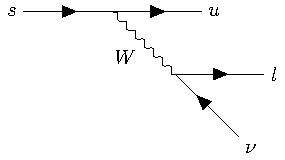
\includegraphics[width=0.4\textwidth]{Images/kaondecay.pdf}
    \caption*{}
    \labfig{kaondecay}
\end{figure}\\
We would like to apply the same tricks used for determining $V_{ud}$ and to do this we need an approximate symmetry that simplifies the analysis. The generalization of isospin to include the strange quark is SU$(3)_{\text{F}}$. The SU(3) symmetry breaking is of order $m_s/\Lambda_{\text{QCD}}\sim20\%$, therefore we expect the precision to be rather poor compared to the precision of our experiments. Moreover, in the measurement of $V_{ud}$, we assumed $f(q^2)\approx f(0)$ since $q^2\ll\Lambda_{\text{QCD}}$. In this case, the kaon and pion masses are much different so the momentum transfer will not be small and, again, this approximation should be very poor.\\
The decays we are interested in are:
\[
K^+\to\pi^0e^+\nu_e \quad K^0\to\pi^-e^+\nu_e
\]
The two decays have different charges, the $K^0$ decay has a spectator $\overline{d}$ quark while the $K^+$ decay has a spectator $\overline{u}$ quark. The two decays are then related by \textbf{isospin}. To the extent that isospin is approximately true, it is sufficient to determine the form factor for only one of these process since the other will be related by symmetry. The matrix element is given by:
\[
\bra{\pi(p_\pi)}\overline{s}\gamma^\mu(1-\gamma_5)u\ket{K(p_K)}=f_+(q^2)(p_\pi+p_K)^\mu+f_-(q^2)q^\mu
\]
Isospin tells us that it is possible to relate the two form factors. $K^0$ is a $\ket{\frac{1}{2},-\frac{1}{2}}$ isospin state, related to $K^+$ by:
\[
J_-\ket{j,m}=\frac{1}{\sqrt{2}}\sqrt{(j+m)(j-m+1)}\ket{j,m-1}
\]
It follows that:
\[
\frac{f_+^{K^+}(0)}{f_+^{K^0}(0)}=\frac{1}{\sqrt{2}}
\]
What about $f_-(q^2)$? Previously, we could use isospin symmetry to explain why this term vanishes in nuclear $\beta$ decay. In the present case, replacing isospin with SU$(3)_{\text{F}}$ does not allow us to neglect $f_-(q^2)$. There is another important argument to neglect it: the contribution of this form factor to the kaon decay is proportional to the lepton mass so for the decays with electrons there is a suppression of a factor $m_e/m_K$. The amplitude associated with this term goes like:
\[
\pazocal{M}(f_-)\sim f_-(q^2)(p_e+p_\nu)_\mu\overline{u}_e\gamma^\mu u_\nu\marginnote{We make use of the fact that:
\[
p_K-p_\pi=p_e+p_\nu
\]}
\]
Contracting now the Lorentz indices gives us:
\[
\pazocal{M}(f_-)\sim f_-(q^2)\overline{u}_e(\slashed{p}_e+\slashed{p}_\nu)u_\nu=f_-(q^2)m_e\overline{u}_eu_\nu\marginnote{Remember that for leptons we have:
\[
\slashed{p}_eu(p_e)=m_eu(p_e) \quad \slashed{p}_\nu u(p_\nu)=0
\]}
\]
\begin{kaobox}[frametitle=Remark]
In pion $\beta$ decay we used isospin symmetry to conclude that $f_-(q^2)=0$. For kaon decay, we observed that SU$(3)_{\text{F}}$ is not as precise as isospin so we found another reason why the contribution mediated by this term is suppressed. A totally legit question would be: \textit{why haven't we applied this reasoning to the pion decay?} For kaon decay, one easily notices that $m_e\ll(m_K-m_\pi)$ which is not true in the case of pion decay, where $m_e$ is not much smaller than $(m_{\pi^+}-m_{\pi^0})$.\\
Another totally legit question is: \textit{would this still work if we considered decays into muons, $K\to\pi\mu\nu$?} Obviously, the answer is no being $m_\mu$ not small compared with $(m_K-m_\pi)$. For semileptonic decays, $f_-(q^2)$ cannot be neglected and instead we are sensitive to it.
\end{kaobox}
To get to this point, we assumed that $q^2\ll\Lambda_{\text{QCD}}$ and that SU(3) breaking is small. These two assumptions manifest into:
\[
f(q^2)=f(0) \quad f(0)=1
\]
Consider the first one. By plotting the decay spectrum with respect to the energy, it turns out that it is a straight line, so the expansion takes the form:
\[
f(q^2)=f(0)+\lambda q^2
\]
where $\lambda\sim0.04$\,fm$^2$ and the higher order terms are not measured. \marginnote{Why should the coefficient be so small? A not-so-satisfactory answer is that to good approximation kaon and pion are point-like. Since the form factors really probe the structure of the particles, the small coefficient is telling us that the process is not sensitive to any meson substructure. As long as $q^2\ll\Lambda_{\text{QCD}}$ this is what we expect.} For $f(0)=1$, the value we find is:
\[
f(0)=0.961\pm0.008
\]
Naively, we would have expected $1\pm20\%$ but instead we got something more like $1\pm4\%$. By playing some numerology, notice that $(20\%)^2=4\%$ which points to the fact that the actual correction is not linear but rather second-order. Somehow, $f(0)=1$ up to second order in SU(3) breaking and this goes under the name of \textbf{Ademollo-Gatto theorem}.\\
This argument does not work for $f_-(q^2)$ but, as mentioned before, there is already a nice suppression on this term. Using the above technique, it is possible to obtain:
\[
V_{us}=0.2257(21)
\]
Moving on from the mesons, another way to measure $V_{us}$ is to look at the decays of \textbf{hyperons}, baryons containing strange quarks and no heavier quarks. As we looked at neutron $\beta$ decay to measure $V_{ud}$, it is possible to measure $\Lambda\to pe\overline{\nu}_e$ in an analogous way to obtain $V_{us}$. Another possibility is to look at the decays of the $\tau$. The $\tau$ is so heavy that its quark decays hadronize, in this sense it is \textit{almost} a hadron. The strategy is to look at the ratio of two decay rates:
\[
\tau^-\to K^-\nu_\tau \quad \tau^-\to\pi^-\nu_\tau
\]
The ratio is simply given by:
\[
R=\frac{\Gamma(\tau^-\to K^-\nu_\tau)}{\Gamma(\tau^-\to\pi^-\nu_\tau)}=\frac{|V_{us}|^2}{|V_{ud}|^2}
\]
The best way to use the $\tau$ is to look at inclusive decays. The main idea is that the $\tau$ is heavy
enough that at $m_\tau$ one can really treat QCD perturbatively. It is possible to calculate how
many light and heavy quarks are produced and trust the perturbative calculation. The inclusive
decay has no form factors, which makes it theoretically very nice, but currently the limiting factor
is the number of experimentally observed $\tau$ decays.
\end{document}